	{\centering
	\chapter{Abstracción}\label{parte3}}
\thispagestyle{empty}
\noindent
\begin{minipage}[t]{0.35\textwidth}
	\begin{flushright}
		{\large
			\vspace{1pt}
			井蛙不可以語於海者，\\
			拘於虛也；\\[0.5em]
			夏蟲不可以語於冰者，\\
			篤於時也；\\[0.5em]
			曲士不可以語於道者，\\
			束於教也。
		}
	\end{flushright}
\end{minipage}%
\hfill
\vrule
\hfill
\begin{minipage}[t]{0.48\textwidth}
	\vspace{1pt}
	\raggedright
	\emph{
		$\!\!$A la rana del pozo no se le puede hablar del mar,\\
		pues está limitada por su espacio.\\[0.5em]
		Al insecto del verano no se le puede hablar del hielo,\\
		pues está restringido por su tiempo.\\[0.5em]
		Al erudito de visión estrecha no se le puede hablar del Dao,\\
		pues está atado por sus enseñanzas.
	}
\end{minipage}

\vspace{1em}
\hfill {   秋水 — \textsc{Zhuāngzǐ, Capítulo 17}}

\section{Comparando adyacencias}
\label{chap:6}
Observando el tablero de dos dimensiones Figura~\ref{fig: tableronm}, podemos notar que este tendrá $xy$ puntos (intersecciones), pero surge la siguiente pregunta: ¿cuántas adyacencias poseen todos esos puntos?
\begin{figure}[H]
	\centering   
	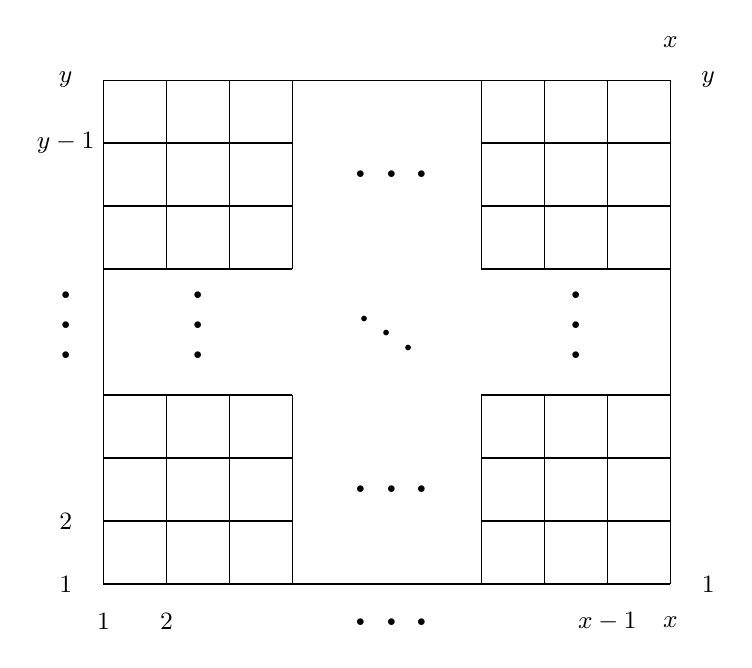
\begin{tikzpicture}[scale=0.8]
		%Cuadrado grande
		\draw (0,0) -- (0,-8);
		\draw (0,0) -- (9,0);
		\draw (9,0) -- (9,-8);
		\draw (0,-8) -- (9,-8);
		%Cuadrado grande
		%Texto horizontal%
		\node(draw)at (0,-8.6) {$1$};
		\node(draw)at (1,-8.6) {$2$};
		\node(draw)at (8,-8.6) {$x-1$};
		\node(draw)at (9,0.6) {$x$};
		\node(draw)at (9.6,0) {$y$};
		
		%Texto vertical%
		\node(draw)at (-0.6,0) {$y$};
		\node(draw)at (-0.6,-1){$y-1$};
		
		\node(draw)at (-0.6,-3.895){\rotatebox{90}{\Huge$\dots$}};
		
		\node(draw)at (-0.6,-7){$2$};
		\node(draw)at (-0.6,-8){$1$};
		%\rotate
		%Lineas para centrar bien
		%\draw (0,-4) -- (9,-4);
		%\draw (4.5,0) -- (4.5,-8);
		%Texto diagonal
		\node(draw)at (9,-8.6) {$x$};
		\node(draw)at (9.6,-8) {$1$};
		\draw[step=1cm] (0,0) grid (3,-3);
		\node(draw)at (1.5,-3.895){\rotatebox{90}{\Huge$\dots$}};
		\node(draw)at (4.526,-3.895) {\rotatebox{-15}
			{\Huge$\ddots$}};
		\node(draw)at (4.573,-8.6) {\Huge$\dots$};
		\node(draw)at (7.5,-3.895) {\rotatebox{90}{\Huge$\dots$}};
		\draw[step=1cm] (0,-5) grid (3,-8);
		\node(draw)at (4.573,-1.5) {\Huge$\dots$};
		\node(draw)at (4.573,-6.5) {\Huge$\dots$};
		\draw[step=1cm] (6,0) grid (9,-3);
		\draw[step=1cm] (6,-5) grid (9,-8);
		
	\end{tikzpicture}
	\caption{Tablero de Go de dimensiones $x\times y$.}
	\label{fig: tableronm}
\end{figure}
Por el Lema~\ref{lem:2n}, estos nodos tienen $2, 3$ o $4$ adyacencias. Los $4$ vértices cuentan con $2$ adyacencias. Hay cuatro aristas, dos de longitud $(x-2)$ y dos de $(y-2)$, cuyos nodos tienen $3$ adyacencias. Además, hay una región interna de $(x-2)(y-2)$ nodos, cada uno con $4$ adyacencias. Esto permite definir la cantidad total de adyacencias de un tablero de $Go^{2}$.

Sea $A(x,y)$ la cantidad total de adyacencias de un tablero de dimensiones $x\times y$. 
\begin{align*}
	A(x,y)&= 2\cdot4 + 3(2(x-2))+3(2(y-2))+4(x-2)(y-2)\\
	A(x,y)&= 8 + 6x-12+6y-12+4xy-8x-8y+16\\
	A(x,y)&= 4xy-2x-2y.
\end{align*}
Definamos también el promedio de adyacencias de un tablero, el cual resulta inmediato de la definición de adyacencias totales; basta dividir por el total de nodos.
Sea $\tilde{A}(x,y)$ la cantidad de libertades promedio de un tablero de dos dimensiones, luego:

\begin{align*}
	\tilde{A}(x,y)= \frac{4xy-2x-2y}{xy}.
\end{align*}
\subsection{El Go en tres dimensiones}

Consideremos el caso para el $Go^3$, de $xyz$ nodos, para esto nos apoyamos en el siguiente esquema, Figura~\ref{fig:3dim_esquema} (izquierda):
\begin{figure}[H]
	\centering
	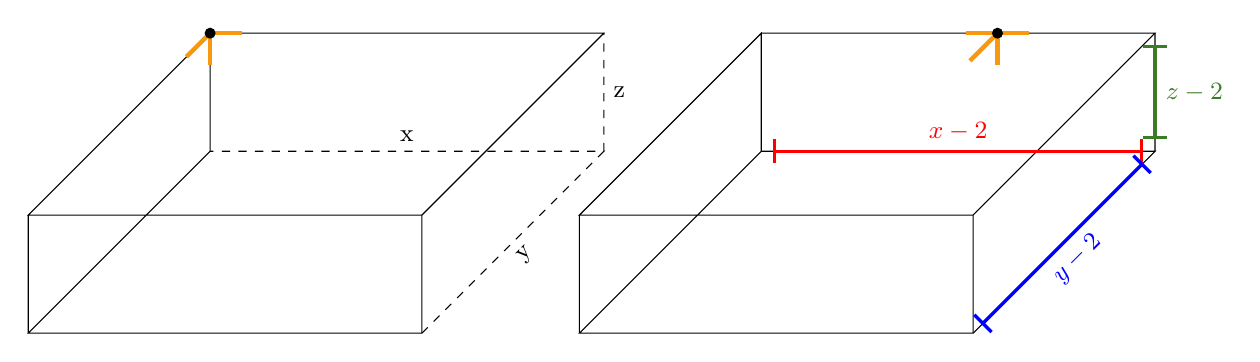
\begin{tikzpicture}[scale=1]
		\pgfmathsetmacro{\x}{-5}
		\pgfmathsetmacro{\y}{6}
		\pgfmathsetmacro{\z}{1.5}
		\path (0,0,\y) coordinate (A) (\x,0,\y) coordinate (B) (\x,0,0) coordinate (C) (0,0,0)
		coordinate (D) (0,\z,\y) coordinate (E) (\x,\z,\y) coordinate (F) (\x,\z,0) coordinate (G)
		(0,\z,0) coordinate (H);
		\draw (A)-- (B)-- (C)--(G)--(F)-- (B) (A)--(E)--(F)--(G)--(H)--(E);
		\draw [dashed,black] (A)--node[below,sloped]{y} (D)-- node[above,sloped]{x}(C) (D)--node[right]{z} (H);
		
		%nodo y sus aristas
		\draw[YellowOrange, ultra thick] (-5,1.5) -- (-5.3,1.2);%adentro
		\draw[YellowOrange, ultra thick]  (-5,1.5) -- (-4.6,1.5);%derecha
		\draw[YellowOrange, ultra thick] (-5,1.5) -- (-5,1.1); %abajo
		
		\fill[color=black] (-5,1.5) circle (0.07);
		\begin{scope}[xshift=7cm]
			\pgfmathsetmacro{\x}{-5}
			\pgfmathsetmacro{\y}{6}
			\pgfmathsetmacro{\z}{1.5}
			\path (0,0,\y) coordinate (A) (\x,0,\y) coordinate (B) (\x,0,0) coordinate (C) (0,0,0)
			coordinate (D) (0,\z,\y) coordinate (E) (\x,\z,\y) coordinate (F) (\x,\z,0) coordinate (G)
			(0,\z,0) coordinate (H);
			\draw (A)-- (B)-- (C)--(G)--(F)--(B) (A)--(E)--(F)--(G)--(H)--(E);
			\draw [black] (A)--(D)--(C) (D)--(H);
			\draw [Red, very thick, |-|](-4.85,0) -- node[above] {$x-2$}(-0.15,0);
			\draw [Blue, very thick, |-|](-0.15,-0.15) -- node[below,sloped] {$y-2$}(-2.2,-2.2);
			\draw [OliveGreen, very thick, |-|](0,1.35) -- node[right] {$z-2$}(0,0.15);
			
			%nodo y sus aristas
			\draw[YellowOrange, ultra thick] (-2,1.5) -- (-2.35,1.15); %adentro
			\draw[YellowOrange, ultra thick]  (-2,1.5) -- (-1.6,1.5); %derecha
			\draw[YellowOrange, ultra thick]  (-2,1.5) -- (-2.4,1.5); %izquierda
			\draw[YellowOrange, ultra thick]  (-2,1.5) -- (-2,1.1);   %abajo
			\fill[color=black] (-2,1.5) circle (0.07);
		\end{scope}
	\end{tikzpicture}
	\caption{Exterior del tablero tres dimensional. Un vértice con $3$ adyacencias, aristas y un nodo con $4$ adyacencias.}
	\label{fig:3dim_esquema}
\end{figure}

Procediendo igual que antes, observamos que este posee $8$ vértices, cada uno con $3$ adyacencias. Identificamos $4$ aristas de $(x-2)$ nodos, $4$ de $(y-2)$ y $4$ de $(z-2)$, cada una con nodos que poseen $4$ adyacencias, véase Figura~\ref{fig:3dim_esquema} (derecha).

%	\begin{figure}[H]
	%		\centering
	%		\begin{tikzpicture}[scale=1.4]
		%			\pgfmathsetmacro{\x}{-5}
		%			\pgfmathsetmacro{\y}{6}
		%			\pgfmathsetmacro{\z}{1.5}
		%			\path (0,0,\y) coordinate (A) (\x,0,\y) coordinate (B) (\x,0,0) coordinate (C) (0,0,0)
		%			coordinate (D) (0,\z,\y) coordinate (E) (\x,\z,\y) coordinate (F) (\x,\z,0) coordinate (G)
		%			(0,\z,0) coordinate (H);
		%			\draw (A)-- (B)-- (C)--(G)--(F)--(B) (A)--(E)--(F)--(G)--(H)--(E);
		%			\draw [dashed,black] (A)--(D)--(C) (D)--(H);
		%			\draw [Red, very thick, |-|](-4.85,0) -- node[above] {$x-2$}(-0.15,0);
		%			\draw [Blue, very thick, |-|](-0.15,-0.15) -- node[below,sloped] {$y-2$}(-2.2,-2.2);
		%			\draw [OliveGreen, very thick, |-|](0,1.35) -- node[right] {$z-2$}(0,0.15);
		%			
		%			%nodo y sus aristas
		%			\draw[YellowOrange, ultra thick] (-2,1.5) -- (-2.35,1.15); %adentro
		%			\draw[YellowOrange, ultra thick]  (-2,1.5) -- (-1.6,1.5); %derecha
		%			\draw[YellowOrange, ultra thick]  (-2,1.5) -- (-2.4,1.5); %izquierda
		%			\draw[YellowOrange, ultra thick]  (-2,1.5) -- (-2,1.1);   %abajo
		%			\fill[color=black] (-2,1.5) circle (0.05);
		%			
		%		\end{tikzpicture}
	%		\caption{Aristas del tablero 3-dimensional y un nodo de 4 adyacencias.}
	%		\label{fig:tablero3d}
	%	\end{figure}

Luego tenemos las caras. Estas se dividen en tres pares: $2$ caras de $(x-2)(y-2)$, $2$ de $(x-2)(z-2)$ y $2$ de $(y-2)(z-2)$, con nodos que poseen $5$ adyacencias cada uno Figura~\ref{fig:3gocaras}.

\begin{figure}[H]
	\centering
	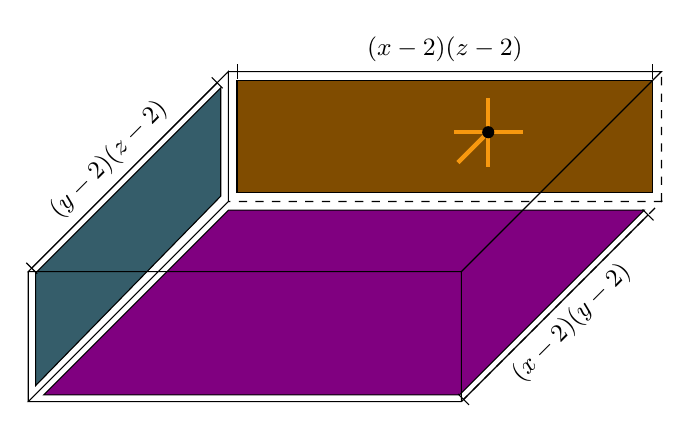
\begin{tikzpicture}[scale=1.1]
		\pgfmathsetmacro{\x}{-5}
		\pgfmathsetmacro{\y}{6}
		\pgfmathsetmacro{\z}{1.5}
		
		%Cara xy
		\filldraw[fill=Blue!50!Red, draw=black] (-0.2,-0.1,0) -- (-5,-0.1,0) -- (-4.9,0,5.8) -- (-0.1,0,5.8) -- cycle;
		
		%Cara yz
		\filldraw[fill=OliveGreen!50!Blue, draw=black](-5.3,-0.2,5) -- (-5.05,0.1,0.1) -- (-5.05,1.35,0.1) -- (-5.3,1.1,5) -- cycle;
		
		%Cara xz
		\filldraw[fill=Red!50!OliveGreen, draw=black] (-0.1,0.1,0) -- (-0.1,1.4,0) -- (-4.9,1.4,0) -- (-4.9,0.1,0) -- cycle;
		
		\draw [black, thin, |-|](-4.9,1.5) -- node[above,sloped] {$(x-2)(z-2)$}(-0.1,1.5);
		\draw [black, thin, |-|](-0.15,-0.15) -- node[below,sloped] {$(x-2)(y-2)$}(-2.29,-2.29);
		\draw [black, thin, |-|](-5.125,1.375) -- node[above,sloped] {$(y-2)(z-2)$}(-7.275,-0.775);
		
		\path (0,0,\y) coordinate (A) (\x,0,\y) coordinate (B) (\x,0,0) coordinate (C) (0,0,0)
		coordinate (D) (0,\z,\y) coordinate (E) (\x,\z,\y) coordinate (F) (\x,\z,0) coordinate (G)
		(0,\z,0) coordinate (H);
		\draw (A)-- (B)--  (C)--(G)--(F)--(B) (A)-- (E)--(F)--(G)--(H)--(E);
		\draw [dashed,black] (A)--(D)--(C) (D)--(H);
		
		
		%nodo y sus aristas
		\draw[YellowOrange, ultra thick] (-2,0.8) -- (-2.4,0.8); %izquierda
		\draw[YellowOrange, ultra thick] (-2,0.8) -- (-1.6,0.8); %derecha
		\draw[YellowOrange, ultra thick]  (-2,0.8) -- (-2,1.2); %arriba
		\draw[YellowOrange, ultra thick] (-2,0.8) -- (-2,0.4); %abajo
		\draw[YellowOrange, ultra thick]  (-2,0.8) -- (-2.35,0.45); %adentro
		\fill[color=black] (-2,0.8) circle (0.07);
		
		
	\end{tikzpicture}
	\caption{Caras del tablero de tres dimensiones con un nodo de $5$ adyacencias.}
	\label{fig:3gocaras}
\end{figure}

Resta el volumen interno, que consiste de $(x-2)(y-2)(z-2)$ nodos, cada uno con $6$ adyacencias. Estamos entonces en condiciones de definir la cantidad total de libertades de un tablero de tres dimensiones.

Sea $A(x,y,z)$ a la cantidad de adyacencias de un  tablero 3-Dimensional, si
\begin{itemize}
	\item$V = 8 \cdot3$, adyacencias de los vértices.
	\item$R =4(4(x-2)+4(y-2)+4(z-2))$, adyacencias de las aristas.
	\item$C=5(2(x-2)(y-2)+2(x-2)(z-2)+2(y-2)(z-2))$, adyacencias de las caras.
	\item$I=6(x-2)(y-2)(z-2)$, adyacencias en el interior.
\end{itemize}
De esta manera, podemos calcular las adyacencias de cualquier tablero de tres dimensiones como sigue,
\begin{align*}
	A(x,y,z)&=V+R+C+I\\
	A(x,y,z)&=6 x y z - 2 x y - 2 x z - 2 y z.
\end{align*}	
Y su promedio,
\begin{align*}
	\tilde{A}(x,y,z)&=\frac{6 x y z - 2 x y - 2 x z - 2 y z}{xyz}.
\end{align*}
A su vez, podemos definir el \textit{exterior} del tablero 3-Dimensional, sea $A(x,y,z)_{\partial}$, la cantidad de adyacencias que tiene el tablero de dimensiones $x,y,z$ que solo toma en cuenta el exterior. Como vimos antes, basta sumar los vértices, las aristas y en caso de las caras, ya no contamos con la adyacencia que va hacia el interior, pues ya no existe al no haber nodos interiores, de modo que nuestras caras tienen 4 adyacencias. Basta tomar $C'= 4(2(x-2)(y-2)+2(x-2)(z-2)+2(y-2)(z-2))$, luego:
\begin{align*}
	A(x,y,z)_{\partial}&=V+A+C'\\
	A(x,y,z)_{\partial}&=8 (x y + x z - 2 x + y z - 2 y - 2 z + 3).
\end{align*}
Definimos inmediatamente el promedio, basta quitar los nodos que no estamos considerando, sea  $\tilde{A}(x,y,z)_{\partial}$ el promedio de libertades del exterior del tablero de dimensiones $x,y,z$:
\begin{align*}
	\tilde{A}(x,y,z)_{\partial}&=\frac{8 (x y + x z - 2 x + y z - 2 y - 2 z + 3)}{(xyz)-(x-2)(y-2)(z-2)}.
\end{align*}
\subsection{Comparando adyacencias promedio}
\label{key:libprom}
Previo a la elaboración de este trabajo, como jugador de Go indagué si existía una versión tridimensional del juego. Al encontrar en Internet únicamente imágenes conceptuales, me pregunté: ¿por qué no desarrollarlo? Así nació \href{https://github.com/10500x/3dGo}{3dGo}. 
\begin{figure}[H]
	\begin{center}
		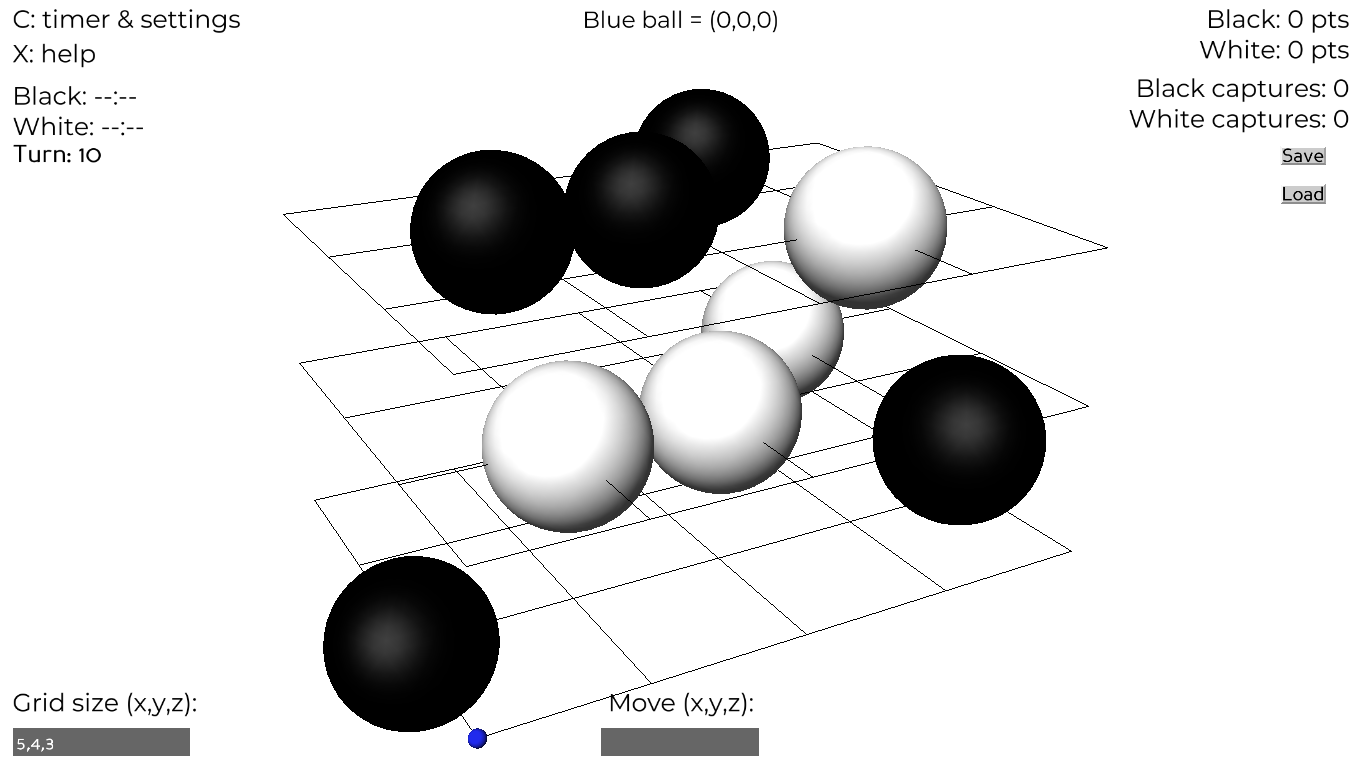
\includegraphics[width=0.9\linewidth]{figures/3dgofoto1}
	\end{center}
	\caption{Tablero de $5\times 4\times 3$ en \href{https://github.com/10500x/3dGo}{3dGo}.}
\end{figure}
Una vez implementadas las reglas, la selección de tamaño del tablero arbitrario y demás opciones noté, junto con quien jugaba, que no se trataba del mismo juego. El 3dGo se sentía más libre, más agresivo. La mayor cantidad de adyacencias alteraba el estilo de juego, diferenciándolo del Go convencional. Para entender esta diferencia, incluso sin experiencia previa, analizaremos el comportamiento del promedio de adyacencias en el límite\footnote{Esta fue la razón de comenzar este escrito.}:

Veamos cuales son los límites de las adyacencias promedio de los tableros de dos y tres dimensiones.
\begin{align*}
	\lim_{x,y\to\infty} \tilde{A}(x,y) &= \lim_{x,y\to\infty} \frac{4xy-2x-2y}{xy} = \lim_{x,y\to\infty} \left( 4 - \frac{2x}{xy} - \frac{2y}{xy} \right) = 4,
\end{align*}
\begin{align*}
	\lim_{x,y,z\to\infty} 
	\tilde{A}(x,y,z)&=\lim_{x,y,z\to\infty}\frac{6 x y z - 2 x y - 2 x z - 2 y z}{xyz}=6.\\
\end{align*}
Es evidente que el promedio de adyacencias en el $Go^{3}$ es considerablemente superior. Esta diferencia se percibe en la experiencia de juego. Surge entonces el problema: ¿Cómo acercar este promedio a $4$? Jugar al $Go^{3}$ debe equivaler a jugar al Go; para ello, debe imitarlo fielmente en reglas, tamaño y sensación de juego.Es por eso que es necesaria esta reducción, porque jugar al $Go^{3}$ no es jugar al $Go^{2}$.

\subsection{Quitar, sí. Pero ¿cómo?}
\label{def_partial}

Como ya vimos, la mayoría de los nodos en el tablero del $Go^{3}$ están en el interior, siempre que el tamaño sea suficientemente grande, donde cada uno tiene $6$ adyacencias. Por ello, la eliminación de nodos debe comenzar por esta región. Le siguen en prioridad las caras ($5$ adyacencias), mientras que las aristas y vértices, al tener $4$ o menos, no afectan el promedio que buscamos. Si tomamos únicamente el exterior del tablero, las caras poseen justamente $4$ adyacencias (perdemos la que va hacia adentro); por lo tanto, analizando su límite, encontramos que:
\begin{align*}
	\lim_{x,y,z\to\infty} \tilde{A}(x,y,z)_{\partial}&=
	\lim_{x,y,z\to\infty}\frac{8 (x y + x z - 2 x + y z - 2 y - 2 z + 3)}{(xyz)-(x-2)(y-2)(z-2)}=4.
\end{align*}
Así, nuestro tablero exterior posee las mismas adyacencias en promedio en el límite, que el $Go^{2}$ es decir: $$\lim_{y,x\to\infty}  \tilde{A}(x,y)= \lim_{x,y,z\to\infty} \tilde{A}(x,y,z)_{\partial}.$$


\subsection{Tablero Toroidal}
\label{key:sectoro}
En el $Go^{2}$, el límite del promedio al hacerlo arbitrariamente grande es 4. Cabe preguntarse: ¿es posible establecer un tablero cuyas libertades promedio sean exactamente 4?

Si unimos los bordes opuestos del tablero obtendremos lo siguiente, Figura~\ref{fig:plano_toro1}

%\begin{wrapfigure}{i}{0.6\textwidth}
\begin{figure}[H]
	\begin{center}
		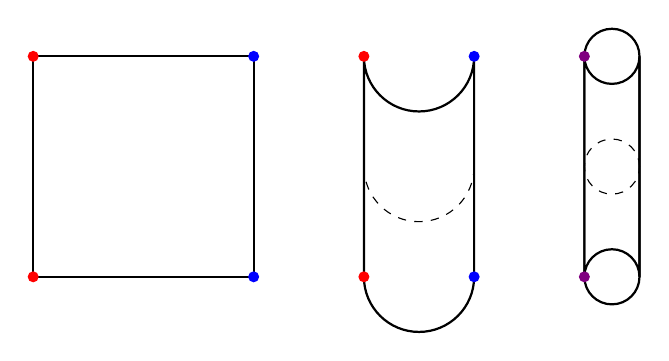
\begin{tikzpicture}[scale=1.4]
			
			% Step 1: Plane (square)
			\draw[thick] (0,0) rectangle (2,2);
			\fill[color=Red] (0,2) circle (0.05);
			\fill[color=Red] (0,0) circle (0.05);
			\fill[color=Blue] (2,0) circle (0.05);
			\fill[color=Blue] (2,2) circle (0.05);
			
			% Step 2: Cylinder
			\begin{scope}[xshift=3cm]
				
				\draw[thick] (0,0) arc[start angle=-180, end angle=0, radius=0.5cm] -- (1,2) arc[start angle=0, end angle=-180, radius=0.5cm] -- cycle;
				
				
				\draw[black, dashed] (1,1) arc[start angle=0, end angle=-180, radius=0.5cm];
				\fill[color=Red] (0,0) circle (0.05);
				\fill[color=Blue] (1,0) circle (0.05);
				\fill[color=Red] (0,2) circle (0.05);
				\fill[color=Blue] (1,2) circle (0.05);
			\end{scope}
			
			\begin{scope}[xshift=5cm]
				\draw[thick] (0,0) arc[start angle=180, end angle=0, radius=0.25cm] -- (.5,2) arc[start angle=0, end angle=180, radius=0.25cm] -- cycle;
				\draw[thick] (0,0) arc[start angle=-180, end angle=0, radius=0.25cm] -- (0.5,2) arc[start angle=0, end angle=-180, radius=0.25cm] -- cycle;
				\fill[color=Red!50!Blue] (0,2) circle (0.05);
				\fill[color=Red!50!Blue] (0,0) circle (0.05);
				\draw[black, dashed] (0.5,1) arc[start angle=0, end angle=360, radius=0.25cm];
				
			\end{scope}
		\end{tikzpicture}
	\end{center}
	\caption{Transición del plano a cilindro al unir sus lados opuestos.}
	\label{fig:plano_toro1}
\end{figure}

Repitamos el proceso, unamos nuestros $4$ vértices, que son ahora $2$, en uno solo, Figura~\ref{fig:plano_toro2}.

%\begin{wrapfigure}[15]{r}{0.57\textwidth}
\begin{figure}[H]
	\begin{center}   
		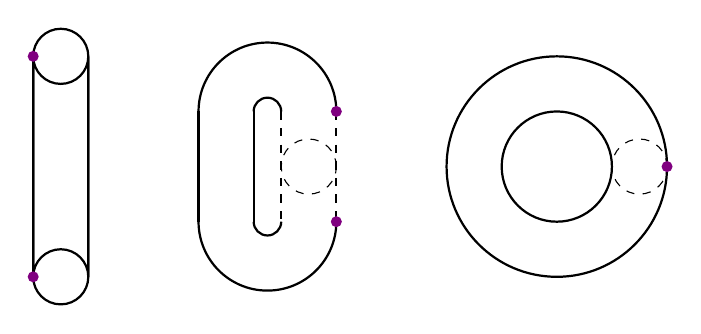
\begin{tikzpicture}[scale=1.4]
			
			%% Cilindro base
			\draw[thick] (0,0) arc[start angle=180, end angle=0, radius=0.25cm] -- (.5,2) arc[start angle=0, end angle=180, radius=0.25cm] -- cycle;
			\draw[thick] (0,0) arc[start angle=-180, end angle=0, radius=0.25cm] -- (0.5,2) arc[start angle=0, end angle=-180, radius=0.25cm] -- cycle;
			\fill[color=Red!50!Blue] (0,2) circle (0.05);
			\fill[color=Red!50!Blue] (0,0) circle (0.05);  
			%\draw[black, dashed] (0.5,1) arc[start angle=0, end angle=360, radius=0.25cm];
			
			
			
			%% Cilindro semi transición
			\begin{scope}[xshift=1.5cm]
				%% Cuerpo de cilindro
				\draw[thick] (0,1.5) -- (0,0.5);
				\draw[thick] (0.5,1.5) -- (0.5,0.5);
				\draw[thick, dashed] (0.75,1.5) -- (0.75,0.5);
				\draw[thick, dashed] (1.25,1.5) -- (1.25,0.5);
				\draw[black, dashed] (1.25,1) arc[start angle=0, end angle=360, radius=0.25cm];
				%%Arcos superiores
				\draw[thick] (0.5,1.5) arc[start angle=180, end angle=0, radius=0.125cm] ;
				\draw[thick](1.25,1.5) arc[start angle=0, end angle=180, radius=0.625cm];
				
				%%Arcos inferiores
				\draw[thick] (0,0.5) arc[start angle=-180, end angle=0, radius=0.625cm] ;
				\draw[thick] (0.5,0.5) arc[start angle=-180, end angle=0, radius=0.125cm] ;
				
				\fill[color=Red!50!Blue] (1.25,1.5) circle (0.05);
				\fill[color=Red!50!Blue] (1.25,0.5) circle (0.05);
				
			\end{scope}
			
			%% Toro
			\begin{scope}[xshift=3.75cm]
				
				%%Circulo externo
				\draw[thick] (0,1) arc[start angle=180, end angle=-180, radius=1cm];
				%%Cirulo interno
				\draw[thick] (0.5,1) arc[start angle=180, end angle=-180, radius=0.5cm];
				%Aristas
				\draw[black, dashed] (2,1) arc[start angle=0, end angle=360, radius=0.25cm];
				%% vértices / vértice
				\fill[color=Red!50!Blue] (2,1) circle (0.05);
				
			\end{scope}
		\end{tikzpicture}
	\end{center}
	\caption{Transición del cilindro al toro tras unir sus caras opuestas.}
	\label{fig:plano_toro2}
\end{figure}
Notemos cómo han cambiado las adyacencias de los vértices, en el plano vimos que eran $2$ para cada uno, pero en el cilindro puede verse que tienen $3$ y más aún en el toro son $4$. Lo mismo ocurre con los nodos en las aristas Figura~\ref{fig:Fig 27}.
%\begin{wrapfigure}{r}{0.6\textwidth}
\begin{figure}[H]
	\begin{center}
		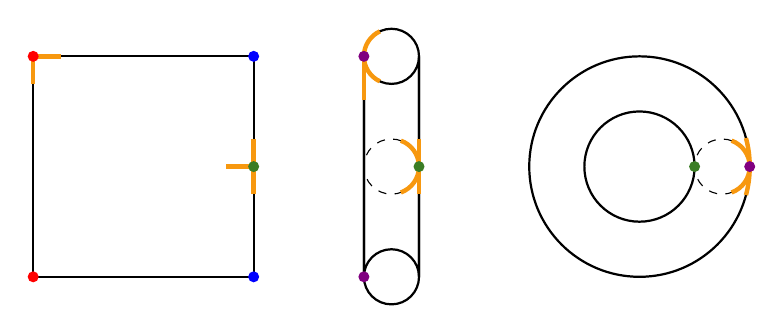
\begin{tikzpicture}[scale=1.4]
			
			% Plano 
			\draw[thick] (0,0) rectangle (2,2);
			
			
			%Libertades nodo rojo
			\draw[YellowOrange, ultra thick] (0,2) -- (0.25,2); %Derecha
			\draw[YellowOrange, ultra thick] (0,2) -- (0,1.75); %Derecha
			%Libertades nodo verde
			\draw[YellowOrange, ultra thick] (2,1) -- (2,1.25);
			\draw[YellowOrange, ultra thick] (2,1) -- (2,0.75);
			\draw[YellowOrange, ultra thick] (2,1) -- (1.75,1);
			
			%nodos
			\fill[color=OliveGreen] (2,1) circle (0.05);
			\fill[color=Red] (0,2) circle (0.05);
			\fill[color=Red] (0,0) circle (0.05);
			\fill[color=Blue] (2,0) circle (0.05);
			\fill[color=Blue] (2,2) circle (0.05);
			
			
			
			
			%% Cilindro 
			\begin{scope}[xshift=3cm]
				
				\draw[thick] (0,0) arc[start angle=180, end angle=0, radius=0.25cm] -- (.5,2) arc[start angle=0, end angle=180, radius=0.25cm] -- cycle;
				\draw[thick] (0,0) arc[start angle=-180, end angle=0, radius=0.25cm] -- (0.5,2) arc[start angle=0, end angle=-180, radius=0.25cm] -- cycle;
				
				
				
				
				%%% vértices Aristas cilindro
				\draw[YellowOrange, ultra thick] (0,2) arc[start angle=-180, end angle=-115, radius=0.25cm];
				\draw[YellowOrange, ultra thick] (0,2) arc[start angle=180, end angle=115, radius=0.25cm];
				\draw[YellowOrange, ultra thick] (0,2) -- (0,1.60); %Abajo
				
				%%% Naranja, libertades y linea punteada
				\draw[YellowOrange, ultra thick] (0.5,1) -- (0.5,1.25);
				\draw[YellowOrange, ultra thick] (0.5,1) -- (0.5,0.75);
				\draw[black, dashed] (0.5,1) arc[start angle=0, end angle=360, radius=0.25cm];
				\draw[YellowOrange, ultra thick] (0.5,1) arc[start angle=0, end angle=70, radius=0.25cm];
				\draw[YellowOrange, ultra thick] (0.5,1) arc[start angle=0, end angle=-70, radius=0.25cm];
				
				%%%% vértices
				\fill[color=Red!50!Blue] (0,2) circle (0.05);
				\fill[color=Red!50!Blue] (0,0) circle (0.05);
				\fill[color=OliveGreen] (0.5,1) circle (0.05);
			\end{scope}
			
			
			%% Toro
			\begin{scope}[xshift=4.5cm]
				%%Circulo externo
				\draw[thick] (0,1) arc[start angle=180, end angle=-180, radius=1cm];
				%%Cirulo interno
				\draw[thick] (0.5,1) arc[start angle=180, end angle=-180, radius=0.5cm];
				
				
				
				%%% Aristas nodo  morado
				\draw[YellowOrange, ultra thick] (2,1) arc[start angle=0, end angle=15, radius=1cm];
				\draw[YellowOrange, ultra thick] (2,1) arc[start angle=0, end angle=-15, radius=1cm];
				\draw[black, dashed] (2,1) arc[start angle=0, end angle=360, radius=0.25cm];
				\draw[YellowOrange, ultra thick] (2,1) arc[start angle=0, end angle=70, radius=0.25cm];
				\draw[YellowOrange, ultra thick] (2,1) arc[start angle=0, end angle=-70, radius=0.25cm];
				
				%% vértices
				\fill[color=Red!50!Blue] (2,1) circle (0.05);
				\fill[OliveGreen] (1.5,1) circle (0.05);
			\end{scope}
			
		\end{tikzpicture}
	\end{center}
	\caption{Cambio de las adyacencias desde el plano al toro.}
	\label{fig:Fig 27} % Assign a unique label
\end{figure}

Vale la pena preguntarse entonces, ¿Es posible hacer esto en cualquier dimensión? Es decir, el llevarlos a su forma «toroidal». Efectivamente es posible y, más aún, es muy sencillo y, a diferencia de la Figura~\ref{fig:Fig 27}, no perdemos puntos.

Bajo nuestra lupa, $G$ solo contiene puntos, el criterio de adyacencia determina sus relaciones. Para relacionar los bordes, basta agregar nuevas relaciones. Lo que buscamos es unir cada cara con su opuesta, a modo de lograr esto, realizamos la siguiente definición, del criterio de adyacencia por opuestos $A_{op}$. Sea $G = N_1 \times \dots \times N_m$, un tablero, donde $|N_k| = n_k$. Diremos que dos puntos $g_1,g_2\in G$ están relacionados opuestamente, si son idénticos en todas sus coordenadas excepto en una, la $k$-ésima, donde toman valores de los extremos:
\begin{equation*}
	g_1=(x_1,\dots, 1, \dots, x_d) \ \sim \ (x_1, \dots, n_k, \dots, x_d)=g_2.
\end{equation*}
Así, de manera tan sencilla, hemos definido el tablero toroidal, que no es más que el mismo tablero que antes, solo que ahora estamos considerando más puntos adyacentes, formalmente, si al criterio canónico le llamamos $A_{ort}$ (adyacencias ortogonales), pasamos de la forma $(G,A_{ort})$, a $(G,A_{ort} \cup A_{op})$.

Es claro que el tablero toroidal tendrá para cada uno de sus nodos $4$ adyacencias. Sea $A(x,y)_{\tau}$ la cantidad de adyacencias del tablero toroidal de tamaño $xy$, realicemos una vez más el proceso que hicimos al principio. El tablero toroidal tendrá; ningún vértice, ningún lado y, en consecuencia, tendrá una sola cara compuesta de $xy$ nodos que, como ya vimos, tendrán $4$ adyacencias por nodo, así.
$$A(x,y)_{T}=4xy.$$
Y su promedio será $4$ pues,
$$A(x,y)_{T}=4xy/xy=4.$$
De esta forma, hemos hallado un tablero tal que para todo nodo, la cantidad de adyacencias es la misma. Hagamos lo mismo en el $Go^{3}$, podemos formular el siguiente esquema, de la Figura~\ref{carasgo3}.

\begin{wrapfigure}{r}{0.5\textwidth}
	%\begin{figure}[H]
	\centering
	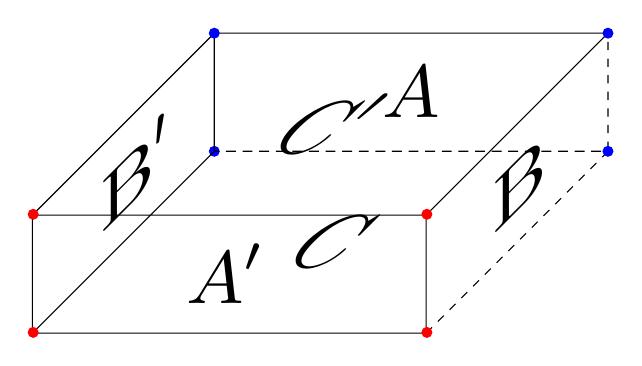
\begin{tikzpicture}[scale=1]
		\pgfmathsetmacro{\x}{-5}
		\pgfmathsetmacro{\y}{6}
		\pgfmathsetmacro{\z}{1.5}
		
		
		%nodo que está atrás
		\fill[color=Blue] (-5,0) circle (0.07);
		
		\path (0,0,\y) coordinate (A) (\x,0,\y) coordinate (B) (\x,0,0) coordinate (C) (0,0,0)
		coordinate (D) (0,\z,\y) coordinate (E) (\x,\z,\y) coordinate (F) (\x,\z,0) coordinate (G)
		(0,\z,0) coordinate (H);
		\draw  (A)-- (B)-- (C)--(G)--(F)-- (B) (A)--(E)--(F)--(G)--(H)--(E);
		\draw [dashed,black] (A)--(D)-- (C)-- (D)--(H);
		
		%nodo y sus aristas
		
		
		\draw (-2.5,0.75) node [thick,scale=3]{$A$};
		\draw (-4.85,-1.55) node [thick,scale=3]{$A'$};
		
		
		
		\draw (-1.15,-0.45) node [thick,scale=3,rotate=0,yslant=1,xslant=-0.25]{$B$};
		\draw (-6,-0.25) node [thick,scale=3,rotate=0,yslant=1,xslant=-0.25]{$B'$};
		
		\draw (-3.5,-1.15) node [thick,scale=3,yslant=0,xslant=0.75]{$C$};
		\draw (-3.5,0.35) node [thick,scale=3,xslant=0.75]{$C'$};
		
		\fill[color=Blue] (-5,1.5) circle (0.07);
		\fill[color=Blue] (0,0) circle (0.07);
		\fill[color=Blue] (0,1.5) circle (0.07);
		
		
		\fill[color=Red] (-7.3,-2.3) circle (0.07);
		\fill[color=Red] (-7.3,-0.8) circle (0.07);
		\fill[color=Red] (-2.3,-0.8) circle (0.07);
		\fill[color=Red] (-2.3,-2.3) circle (0.07);
		
	\end{tikzpicture}
	\caption{Caras del $Go^{3}$.}
	\label{carasgo3}
\end{wrapfigure}

Aquí, si aplicamos la nueva relación, obtenemos que todos los puntos tendrán $6$ adyacencias. Pues los vértices obtendrán $3$ nuevas adyacencias, llevándolas a $6$, los lados obtendrán $2$ nuevas adyacencias, llevándolos a $6$. Finalmente las caras obtienen una sola adyacencia nueva, la opuesta. Obteniendo así la igualdad en el límite.

Ahora bien ¿qué pasaría si tomamos en cuenta solo los puntos que están en el borde? 

\noindent
Si $x\in G, x=(x_1,\dots,x_n)$ con, $x_i \leq k_i=|n_i|$, el borde será el de los puntos dados por $G'=\{x\in G: \exists i, (x_i= 1 \lor x_i =n_i) \}$.

A través del criterio de adyacencia canónico, obtenemos un tablero que es tal que posee en su límite $4$ adyacencias por punto, pues tan solo los vértices poseen $3$ adyacencias, lo que vimos en la Sección~\ref{def_partial}.

Si a este tablero le adjuntamos las adyacencias dadas por el criterio por opuestos, obteniendo $(G',A\cup A_o)$. Tendrá $5$ adyacencias para todo punto, pues al carecer de los puntos interiores, las caras, pierden una adyacencia, pero la ganan a través de la cara opuesta. los bordes, que poseen $4$ adyacencias, ganan $2$ y los vértices obtienen $3$. Como las caras representan la mayor cantidad de puntos, es claro que su límite será $5$, claro está, llevado a tamaños grandes.

Si recordamos el Lema~\ref{lem:2n}. Al realizar estos procedimientos a un tablero cualquiera, siempre podemos llegar a la igualdad de $2n$ adyacencias por punto. Pues el criterio por opuestos garantiza llenar todas las adyacencias faltantes. Es fácil ver que, al tomar tableros arbitrariamente grandes, cualquier tablero de n dimensiones posee en el límite $2n$ adyacencias promedio. 

Para este problema, para $n=2$, $A_{ort}$ proporciona una solución al caso de grado lo más cercano a 4, mientras que la relación $\mathcal{A} = A_{ort} \cup A_{{op}}$ satisface la condición de grado exactamente 4. Además, para el caso $ n = 3 $, fuimos capaces de hallar una solución parcial sobre el borde: si $G' = \{ x \in G \mid \exists i \text{ tal que } (x_i = 1 \lor x_i = n_i) \}$ denota la frontera, entonces el grafo $(G', \mathcal{A} )$ es una solución para el caso de grado lo más cercano posible a 4 sobre la superficie.

%	Veamos una solución general. Para forzar 4 adyacencias en $n \ge 2$ manteniendo la estructura original de $G$, aprovechamos que el grado de un vértice en un producto cartesiano de grafos es la suma de los grados de sus factores. Dado que un ciclo $C_k$ es exactamente 2-regular, el producto cartesiano de exactamente dos ciclos ($C_a \times C_b$) siempre resultará en un grafo 4-regular. La estrategia consiste en colapsar las $n$ dimensiones en exactamente dos «meta-dimensiones''.
%		
%			Sea $G = N_1 \times \cdots \times N_n$, con $n \ge 3$. Particionamos el conjunto de índices $\{1, 2, \dots, n\}$ en dos subconjuntos disjuntos y no vacíos, $I$ y $J$. 
%			
%			Definimos dos nuevos conjuntos basados en el producto cartesiano de los $N_i$ correspondientes:
%			\begin{equation*}
	%				U = \prod_{i \in I} N_i \quad \text{y} \quad V = \prod_{j \in J} N_j
	%			\end{equation*}
%			Existe una biyección natural entre $G$ y $U \times V$. Sean $m_U = |U|$ y $m_V = |V|$. 
%			Para dotar a $U$ y $V$ de una estructura de ciclo, establecemos biyecciones hacia grupos cíclicos mediante el orden lexicográfico: $\phi_U: U \to \mathbb{Z}_{m_U}$ y $\phi_V: V \to \mathbb{Z}_{m_V}$.
%			
%			Construimos la familia $\mathcal{A}' = \{R_U, R_V\}$ sobre $G \cong U \times V$:
%			\begin{itemize}
	%				\item \textbf{Relación $R_U$ (Ciclo en la primera meta-dimensión):}
	%				\begin{equation*}
		%					R_U = \{ ((u,v), (u',v)) \in G \times G \mid \phi_U(u) \equiv \phi_U(u') \pm 1 \pmod{m_U} \}
		%				\end{equation*}
	%				\item \textbf{Relación $R_V$ (Ciclo en la segunda meta-dimensión):}
	%				\begin{equation*}
		%					R_V = \{ ((u,v), (u,v')) \in G \times G \mid \phi_V(v) \equiv \phi_V(v') \pm 1 \pmod{m_V} \}
		%				\end{equation*}
	%			\end{itemize}
%	Obtenemos $H = (G, R_U \cup R_V)$ es conexo, simple (siempre que $m_U \ge 3$ y $m_V \ge 3$), y estrictamente 4-regular para cualquier $n$.
%		
\newpage
\section{El Go en una dimensión}\label{Go_1dim}
%\begin{figure}[H]
\begin{wrapfigure}[5]{r}{0.4\textwidth}
	\centering
	\begin{tikzpicture}[scale=0.7]
		% Draw the background
		\fill[goban] (-0.5,-0.5) rectangle (6.5,0.5);
		
		% Draw the grid lines
		\draw (0,0) -- (6,0);
		\draw (0,-0.25) -- (0,0.25);
		\draw (1,-0.2) -- (1,0.2);
		\draw (2,-0.2) -- (2,0.2);
		\draw (3,-0.2) -- (3,0.2);
		\draw (4,-0.2) -- (4,0.2);
		\draw (5,-0.2) -- (5,0.2);
		\draw (6,-0.25) -- (6,0.25);
		% Draw the central black dot
		
		\begin{scope}[yshift=-1.5cm]
			\fill[goban] (-0.5,-0.5) rectangle (6.5,0.5);
			
			% Draw the grid lines
			\draw (0,0) -- (6,0);
			\draw (0,-0.25) -- (0,0.25);
			\draw (1,-0.2) -- (1,0.2);
			\draw (2,-0.2) -- (2,0.2);
			\draw (3,-0.2) -- (3,0.2);
			\draw (4,-0.2) -- (4,0.2);
			\draw (5,-0.2) -- (5,0.2);
			\draw (6,-0.25) -- (6,0.25);
			
			\filldraw[black] (4,0) circle (10pt);
			\path (4,0) node [white]{1};
			
			\filldraw[draw=black,fill=white] (2,0) circle (10pt);
			\path (2,0) node [black]{2};
		\end{scope}
		
	\end{tikzpicture}
	\caption{Tablero vacío y, tablero con una piedra negra y una blanca.}
	\label{fig:1dim_go}
\end{wrapfigure}
Primero veamos cómo se ve Figura~\ref{fig:1dim_go}. Claramente hay dos libertades por punto, excepto en los bordes, que cuentan con una. Por lo tanto,
\begin{align*}
	A(n)&=2*1+(n-2)*2=2n-2.\\
	\tilde{A}(n)&=\frac{2n-2}{n}=2-\frac{2}{n}.
\end{align*}
Luego, es claro que en el límite de su promedio es $2$.

\label{teoremas_go1}
\begin{lemma}
	En el $Go^{1}$, canónico, las únicas regiones que pueden constituir un ojo son los puntos extremos del tablero, toda otra región vital es una unión.
\end{lemma}
\begin{proof}
	Por definición, un ojo para un grupo es una región vital rodeada completamente por un único grupo $I$. Sea $R$ una región, para que $I$ rodee a $R$, y sea vital, su frontera $\partial R$ debe pertenecer a $I$.
	\begin{figure}[H]
		\centering
		\begin{tikzpicture}[scale=0.7]
			% Draw the background
			\fill[goban] (-0.5,-0.5) rectangle (6.5,0.5);
			
			% Draw the grid lines
			\draw (0,0) -- (6,0);
			\draw (0,-0.25) -- (0,0.25);
			\draw (1,-0.2) -- (1,0.2);
			\draw (2,-0.2) -- (2,0.2);
			\draw (3,-0.2) -- (3,0.2);
			\draw (4,-0.2) -- (4,0.2);
			\draw (5,-0.2) -- (5,0.2);
			\draw (6,-0.25) -- (6,0.25);
			\filldraw[black] (3,0) circle (10pt);
			\filldraw[black] (5,0) circle (10pt);
			
			
			\filldraw[draw=black,fill=white] (1,0) circle (10pt);
			
			\fill[draw=black,fill=purple, very thin] (-0.25,-0.25) rectangle (0.25,0.25);
			\fill[draw=black,fill=cyan, very thin] (3.75,-0.25) rectangle (4.25,0.25);
			
		\end{tikzpicture}
		\caption{\textcolor{purple}{Ojo} en el borde, \textcolor{cyan}{unión} en el interior.}
		\label{fig:ej_go1dim}
	\end{figure}
	\paragraph{$R$ en el interior:}
	Por el lema \ref{lem:2n}, si $x\in R$, posee dos adyacencias: $x-1$ y $x+1$. 
	
	Para que $x$ sea ojo de $I$, debe cumplirse que $\{(x-1, e), (x+1, e)\} \subset I$. Al ser $I$ conexo, existiría un camino en $I$ entre $x-1$ y $x+1$. Sin embargo, la forma del tablero obliga a pasar por $x$, que está vacío, por lo que tal camino no existe.
	
	En consecuencia, $x-1$ y $x+1$ están desconectados y no pueden pertenecer al mismo grupo $I$. Una región en el interior está siempre rodeada por dos grupos distintos. A lo sumo, puede darse que $\partial R$ esté dado pos dos grupos de un mismo color, luego es una unión. 
	
	\paragraph{$R$ en el borde:}
	Si $x = 1$, su única adyacencia es el punto $2$. Si un grupo $I$ posee una piedra en $2$, entonces la totalidad de la frontera de $x$ pertenece a $I$. Por lo tanto $x$ es vital para $I$ y, al ser que hay un solo grupo que rodea a $x$, $x$ es un Ojo para $I$. El caso $x=n$ es análogo.
\end{proof}
\section{Hallando el origen en común}

Hasta ahora, hemos construido el Go bidimensional y explorado sus generalizaciones a una y tres dimensiones. Aunque sus dinámicas difieren, surge una pregunta natural: ¿se trata realmente de estructuras distintas? Veremos que todas ellas pueden obtenerse a partir de un mismo origen.

Un juego de Go queda determinado por una estructura $(G,E,A,\Delta)$. Para relacionar distintas variantes, introduciremos ciertas aplicaciones naturales que permiten construir unas variantes a partir de otras preservando las adyacencias y las reglas del juego.

Para dotar de dimensión a un conjunto de nodos, definimos la aplicación
$$\phi:(G,E,A,\Delta)\to(G\times\{1\},E,A,\Delta).$$
Dada por $\phi(g)=(g,1)$.
La preservación de la adyacencia es inmediata, además, $\phi$ es inyectiva.
$$\phi(g_1)\sim\phi(g_2)\iff(g_1,1)\sim(g_2,1).$$
Para expandir el tablero con un conjunto $M$ hacemos uso de la aplicación
$$\Xi:(G,E,A,\Delta)\to(G\times M,E,A,\Delta).$$
Fijando una coordenada $m \in M$, definimos $\Xi(g) = (g,m)$. Nuevamente, la adyacencia se conserva y es inyectiva, ya que $(g_1,m) = (g_2,m) \implies g_1 = g_2$.:
$$\Xi(g_1) \sim \Xi(g_2) \iff (g_1,m) \sim (g_2,m).$$
Para incorporar jugadores adicionales, definimos una inclusión $$\iota: (G,E,A,\Delta) \to (G,E \cup \{y\},A,\Delta).$$ Con $y \notin E$, tal que $\iota(e) = e$ para todo $e \in E$. 

Es inyectivo ($\iota(e_1) = \iota(e_2) \Rightarrow e_1 = e_2$) y preserva la identidad de los estados previos. Por diseño no es sobreyectivo, para poder acomodar el nuevo elemento.


Consideremos $Go^0_0 = (\{1\}, \{0\}, A, \Delta)$, un juego de un solo nodo sin jugadores. Sabiendo que $\{1\} \times N \cong_A N$, obtenemos el siguiente diagrama (Figura~\ref{fig:familia-go}).
\begin{figure}[H]
	\centering
	\begin{tikzcd}
		{Go_0^0} && {Go_1^0} && {Go_m^0} \\
		\\
		{Go_0^1} && {Go_1^1} && {Go_m^1} \\
		\\
		{Go_0^n} && {Go_1^n} && {Go_m^n}
		\arrow["id"{description}, from=1-1, to=1-1, loop, in=215, out=145, distance=10mm]
		\arrow["\iota", hook, from=1-1, to=1-3]
		\arrow["\Xi", hook, from=1-1, to=3-1]
		\arrow[dashed, from=1-1, to=3-3]
		\arrow["\dots", hook, from=1-3, to=1-5]
		\arrow["\Xi", hook, from=1-3, to=3-3]
		\arrow["\Xi", hook, from=1-5, to=3-5]
		\arrow["\iota", hook, from=3-1, to=3-3]
		\arrow["\vdots", hook, from=3-1, to=5-1]
		\arrow["\dots", hook, from=3-3, to=3-5]
		\arrow["\vdots", hook, from=3-3, to=5-3]
		\arrow[dashed, from=3-3, to=5-5]
		\arrow["\vdots", hook, from=3-5, to=5-5]
		\arrow["\iota"', hook, from=5-1, to=5-3]
		\arrow["\dots"', hook, from=5-3, to=5-5]
	\end{tikzcd}
	\caption{Estructura de la familia de \textit{Juegos de Go}. A derecha agregamos jugadores, hacia abajo expandimos el tablero.}
	\label{fig:familia-go}
\end{figure}
Al recordar a 老子 — \textit{Lao Tse}, redescubrimos lo ya dicho:\\
\noindent
\begin{minipage}[t]{0.35\textwidth}
	\begin{flushright}
		{\large
			\vspace{1pt}
			道生一，\\
			一生二，\\
			二生三，\\
			三生万物。
		}
	\end{flushright}
\end{minipage}%
\hfill
\vrule
\hfill
\begin{minipage}[t]{0.48\textwidth}
	\raggedright
	\vspace{1pt}
	\emph{
		$\ \!\!\!$El Tao engendra al Uno.\\
		El Uno engendra al Dos.\\
		El Dos engendra al Tres.\\
		El Tres engendra las diez mil cosas.}
\end{minipage}

\vspace{1pt}
\hfill  道德經 — {\textsc{Dàodé jīng Capítulo 42}}\\

Podemos ir un poco más lejos, si recordamos lo visto en el Sección~\ref{key:sectoro}, podemos definir una transformación natural que asocia a cada tablero plano su versión toroidal.

Esta aplicación no altera la cantidad de nodos ni de jugadores; únicamente modifica las relaciones de adyacencia, identificando posiciones opuestas del tablero.

Definimos entonces la aplicación toroidal
\[\tau:(G,E,A,\Delta)\to(G,E,A\cup A_o,\Delta),\]
donde $A$ es la relación de adyacencia original y $A_o$ la relación entre posiciones opuestas.
La aplicación actúa como la identidad sobre los nodos. Además,
\[g_1\sim_A g_2\implies\tau(g_1)\sim_{A\cup A_o}\tau(g_2).\]
Como $A\subseteq A\cup A_o$, esta propiedad es inmediata. En particular, $\tau$ es inyectiva.

Por otra parte, recordando el análisis de las adyacencias realizado en la Sección~\ref{chap:6}, observamos que las posiciones del borde poseen un comportamiento distinto al de las posiciones interiores. Para aislar este fenómeno introducimos la aplicación de frontera
\[\partial:(G,E,A,\Delta)\to(\partial G,E,A,\Delta),\]
Donde $\partial G = \{ x \in G : \exists i, x_i = 1 \text{ o } x_i = n_i \}$, tal como lo definimos en el Sección~ \ref{key:sectoro}.
\subsection*{El Toro Hueco}
Combinando ambas construcciones, nos permite construir el diagrama de la Figura~\ref{fig: torohueco}. 

\begin{figure}[H]
	\centering
	\begin{tikzcd}
		{Go_0^0} && {Go^{n}_{m}} \\
		\\
		{\partial T_0^0} && {\partial T_n^m}
		\arrow["{\Xi, \iota}", hook, from=1-1, to=1-3]
		\arrow["{\tau, \partial}"', maps to, from=1-1, to=3-1]
		\arrow[dashed, from=1-1, to=3-3]
		\arrow["{\tau, \partial}", maps to, from=1-3, to=3-3]
		\arrow["{\Xi, \iota}"', hook, from=3-1, to=3-3]
	\end{tikzcd}
	\caption{Diagrama de la estructura completa. Las flechas horizontales ($\Xi$) expanden dimensiones y jugadores ($\iota$). Las verticales ($\tau$) cierran el espacio y ($\partial$) vacían el interior.}
	\label{fig: torohueco}
\end{figure}

%\begin{theorem}
%	En el $Go^{1}_{2}$ y en ausencia de komi. Existe una estrategia óptima donde el primer jugador siempre gana ó empata.
%\end{theorem}
%
%
%Sea $n$ el tamaño del tablero. Antes de ver el caso general, veamos los casos más importantes, los pequeños.
%
%\begin{figure}[H]
%	\centering
%	\begin{tikzpicture}[scale=0.7]
	%		% Draw the background
	%		\fill[goban] (-0.25,-0.5) rectangle (0.75,0.5);
	%		% Draw the grid lines
	%		\draw (0.25,-0.25) -- (0.25,0.25);
	%		
	%		\begin{scope}[xshift=2cm]
		%			\fill[goban] (-0.25,-0.5) rectangle (1.25,0.5);
		%			% Draw the grid lines
		%			\draw (0,-0.25) -- (0,0.25);
		%			\draw (0,0) -- (1,0);
		%			\draw (1,-0.25) -- (1,0.25);
		%		\end{scope}
	%		
	%		
	%		\begin{scope}[xshift=4.5cm]
		%			\fill[goban] (-0.25,-0.5) rectangle (2.25,0.5);
		%			% Draw the grid lines
		%			\draw (0,-0.25) -- (0,0.25);
		%			\draw (0,0) -- (2,0);
		%			\draw (1,-0.2) -- (1,0.2);
		%			\draw (2,-0.25) -- (2,0.25);
		%			\filldraw[black] (1,0) circle (10pt);
		%		\end{scope}
	%	\end{tikzpicture}
%	\caption{Estrategia óptima en $Go^{1}_{2}$ de tamaño $1$,$2$ y $3$.}
%\end{figure}
%
%\paragraph{$n=1:$}
%Aquí, el negro no puede jugar, pues el punto no tiene libertades, por lo tanto, negro pasa. blanco se encuentra en la misma situación, pasa y la partida termina en empate.
%\paragraph{$n=2:$}
%Aquí, si negro juega en algún punto, blanco lo captura en el turno siguiente, luego negro no puede recapturar, por regla del ko. Por lo tanto, la mejor jugada es pasar, blanco pasa también, pues concluye lo mismo, empate.
%\paragraph{$n=3:$}
%La única jugada ganadora es jugar en el medio, blanco no puede jugar, pues ambas posibles jugadas son suicidio, blanco pasa, negro pasa. negro gana por $2$ puntos.
%\paragraph{$n=4:$}
%Aquí empezamos a notar que para $n$ par, la estrategia óptima es la misma si se juega de un lado del tablero que del otro, pues por la simetría del tablero, resulta un espejo del otro. Sin importar donde juegue blanco, siempre le queda una libertad, con lo cual es comido al turno siguiente. negro gana.
%\paragraph{$n=5:$}
%Igual que en $n=4$, donde sea que juegue el blanco, va a tener una libertad, negro toma al siguiente turno, así hasta que blanco no pueda jugar por ko. negro gana.
%\begin{figure}[H]
%	\centering
%	\begin{tikzpicture}[scale=0.7]
	%		\fill[goban] (-0.25,-0.5) rectangle (3.25,0.5);
	%		% Draw the grid lines
	%		\draw (0,-0.25) -- (0,0.25);
	%		\draw (0,0) -- (3,0);
	%		\draw (1,-0.2) -- (1,0.2);
	%		\draw (2,-0.2) -- (2,0.2);
	%		\draw (3,-0.25) -- (3,0.25);
	%		\filldraw[black] (1,0) circle (10pt);
	%		\begin{scope}[xshift=4cm]
		%			\fill[goban] (-0.25,-0.5) rectangle (3.25,0.5);
		%			% Draw the grid lines
		%			\draw (0,-0.25) -- (0,0.25);
		%			\draw (0,0) -- (3,0);
		%			\draw (1,-0.2) -- (1,0.2);
		%			\draw (2,-0.2) -- (2,0.2);
		%			\draw (3,-0.25) -- (3,0.25);
		%			\filldraw[black] (2,0) circle (10pt);
		%		\end{scope}
	%		\begin{scope}[xshift=8cm]
		%			\fill[goban] (-0.25,-0.5) rectangle (4.25,0.5);
		%			\draw (0,0) -- (4,0);
		%			% Draw the grid lines
		%			\draw (0,-0.25) -- (0,0.25);
		%			\draw (1,-0.2) -- (1,0.2);
		%			\draw (2,-0.2) -- (2,0.2);
		%			\draw (3,-0.2) -- (3,0.2);
		%			\draw (4,-0.25) -- (4,0.25);
		%			\filldraw[black] (2,0) circle (10pt);
		%		\end{scope}
	%	\end{tikzpicture}
%	\caption{Estrategia óptima en tamaño $4$ y $5$.}
%\end{figure}
%
%La estrategia óptima consiste en jugar en el centro del tablero, para $n$ impar dicho centro siempre existe y para $n$ par, jugamos en alguno de los dos puntos que están lo más próximo al centro. Decimos que es óptimo, pues al jugar en el centro o lo más cerca posible, logramos partir el tablero en dos, dichos dos subtableros tienen influencia del negro, con lo cual, aunque el blanco sea capaz de asegurar la mayor cantidad de territorio posible en uno de los lados, jamás va a poder ser capaz de controlar todo el territorio, pues hay un punto que estará en conflicto con el blanco. Así, basta que el negro juegue en el otro lado de manera tal de asegurar la misma cantidad de puntos que el blanco, como el negro tiene la influencia en el centro, este tendrá un punto más dado por el borde del subtablero que está siendo controlado por el negro. Así estamos seguros de que el negro o bien tiene más puntos o bien empata con el blanco, para todo tamaño.
%
%En general, la estrategia óptima esta dada por la siguiente función:
%
%$$
%f(t) = \begin{cases} 
	%	(b, k'): P(k')\sim k   \wedge C(k')=0 & \text{si } (A) \text{ (Captura)} \\
	%	(n, n - k + 1) & \text{si } (B) \text{ (Espejo)} \\
	%	\varnothing & \text{si } (C) \text{ (Fin)}
	%\end{cases}
	%$$
	%
	%Donde los casos se evalúan en orden de prioridad:
	%
	%\paragraph{(A) Ataque:} Si la jugada del blanco es la piedra de posición $P(i_k)=k$ resulta un ataque es decir, $k$ es adyacente a un grupo negro $I_k(1)$, $2 \in C(R(I_k(1)))$. respondemos capturando inmediatamente en la única libertad restante ($k+1$ o $k-1$).
	%
	%\paragraph{(B) Espejo:} Si blanco realiza una jugada que no ataca, basta realizar la misma jugada pero espejada. Esto mantiene la paridad territorial.
	%
	%\paragraph{(C) Fin:} Si el blanco decide pasar su turno ($f(t-1) = \varnothing$), nosotros también pasamos para terminar la partida y asegurar la victoria por puntos.
	%
	%A modo de hacer más sencilla la lectura de la estrategia óptima, hemos realizado un diagrama de flujo:
	%
	%\begin{figure}[H]
	%	\centering
	%	\begin{tikzpicture}[
		%		node distance=2cm, 
		%		auto,
		%		% Estilos
		%		start/.style={rectangle, rounded corners, minimum width=3cm, minimum height=1cm, text centered, draw=black, fill=gray!10},
		%		decision/.style={diamond, minimum width=3cm, minimum height=1cm, text centered, draw=black, aspect=2.5},
		%		process/.style={rectangle, minimum width=3cm, minimum height=1cm, text centered, draw=black},
		%		arrow/.style={thick, ->, >=stealth},
		%		note/.style={text width=3cm, align=right, font=\footnotesize, color=black}
		%		]
		%		
		%		% --- ESTRUCTURA CENTRAL ---
		%		
		%		% Nodo Inicio
		%		\node (start) [start] {blanco realiza la jugada $f(t-1)$};
		%		
		%		% Decisión 1: ¿Es Ataque?
		%		\node (dec1) [decision, below=1.5cm of start] {¿Es un ataque?};
		%		\node (dec2) [decision, below=1.5cm of dec1] {¿blanco en el borde?};
		%		% Decisión 2: ¿blanco Pasó? (Nueva lógica)
		%		\node (dec3) [decision, below=1.5cm of dec2] {¿blanco Pasó?};
		%		
		%		% Acción Final: Espejo (Respuesta por defecto ante cualquier jugada no agresiva)
		%		\node (proc3) [process, below=1.5cm of dec3] {\textbf{Espejo}};
		%		\node (desc3) [below=0.1cm of proc3, font=\footnotesize] {Jugar simétrico en $n-k+1$};
		%		
		%		
		%		% --- NOTAS EXPLICATIVAS (Izquierda) ---
		%		
		%		\node [note, left=0.5cm of dec1] (note1) {\textit{¿$2 \in C(R(I_j(1)))$?}\\(blanco juega adyacente a negro)};
		%		\node [note, left=0.5cm of dec2] (note2) {\textit{
				%				¿$P(f(t-1))=1$ ó\\ $P(f(t-1))=n$ ?}};
		%		\node [note, left=0.5cm of dec3] (note2) {\textit{¿$f(t-1)= \varnothing$?\\ blanco pasa}};
		%		
		%
		%		% --- RAMA Derecha ---
		%		% Acción 1: Captura
		%		\node (proc1) [process, right=2cm of dec1] {\textbf{Capturar}};
		%		\node [note, below=0.1cm of proc1] (desc1) {Jugar en $(b,k'): P(k')\sim P(k)$ y $C(k')=0$.};
		%		
		%		% Acción 2: Pasar
		%		\node (proc2) [process, right=1.5cm of dec2] {\textbf{Capturar}};
		%		\node (desc2) [below=0.1cm of proc2, font=\footnotesize] {$P(f(t))=2$ ó $n-1$};
		%		\node (proc4) [process, right=1.5cm of dec3] {\textbf{Pasar}};
		%		\node (desc3) [below=0.1cm of proc4, font=\footnotesize] {$f(t)=\varnothing$ ó $n-1$};
		%		
		%		
		%		% --- CONEXIONES ---
		%		
		%		\draw [arrow] (start) -- (dec1);
		%		
		%		% Flechas Decisión 1 (Ataque)
		%		\draw [arrow] (dec1) -- node[anchor=south, near start] {Sí} (proc1);
		%		\draw [arrow] (dec1) -- node[anchor=east] {No} (dec2);
		%		
		%		% Flechas Decisión 2 (Pase)
		%		\draw [arrow] (dec2) -- node[anchor=south, near start] {Sí} (proc2);
		%		\draw [arrow] (dec2) -- node[anchor=east] {No} (dec3);
		%		\draw [arrow] (dec3) -- node[anchor=east] {No} (proc3);
		%		\draw [arrow] (dec3) -- node[anchor=south] {Si} (proc4);
		%		
		%	\end{tikzpicture}
	%	\caption{Diagrama de flujo de la estrategia para el $Go^{1}_{2}$.}
	%	\label{fig:flowchart_go1_v2}
	%\end{figure}
	%
	%Expliquemos qué queremos decir que la estrategia es jugar en el centro.
	%
	%\subsubsection{Caso Impar}
	%\begin{figure}[H]
	%	\centering
	%	\begin{tikzpicture}[scale=0.7]
		%		% Background (Ajustado a 18.5 para igualar la Figura~anterior)
		%		\fill[goban] (-0.5,-0.5) rectangle (18.5,0.5);
		%		
		%		% --- Bloque Izquierdo (0-4) ---
		%		\draw (0,0) -- (4,0);
		%		\draw (0,-0.25) -- (0,0.25); % Borde Inicio
		%		\foreach \x in {1,2,3,4} \draw (\x,-0.2) -- (\x,0.2);
		%		
		%		% Puntos suspensivos
		%		\foreach \x in {4.5, 5.0, 5.5} \path (\x,0) node [black]{.};
		%		
		%		% --- Bloque Central (6-12) ---
		%		\draw (6,0) -- (12,0);
		%		\foreach \x in {6,...,12} \draw (\x,-0.2) -- (\x,0.2);
		%		
		%		% PIEDRAS (Centro en 9)
		%		\filldraw[OliveGreen] (8,0) circle (3pt);
		%		\filldraw[black] (9,0) circle (10pt); % Piedra Central
		%		\filldraw[OliveGreen] (10,0) circle (3pt);
		%		
		%		% Puntos suspensivos
		%		\foreach \x in {12.5, 13, 13.5} \path (\x,0) node [black]{.};
		%		
		%		% --- Bloque Derecho (14-18) ---
		%		% (Extendido hasta 18 para igualar ancho total)
		%		\draw (14,0) -- (18,0);
		%		\foreach \x in {14,...,18} \draw (\x,-0.2) -- (\x,0.2);
		%		\draw (18,-0.25) -- (18,0.25); % Borde Final
		%		
		%	\end{tikzpicture}
	%	\caption{Tablero de $Go(n)$ e influencia de la piedra Negra inicial}
	%\end{figure}
	%Si jugamos exactamente en el centro, habremos dividido el tablero en dos tableros casi iguales, ambos de $\frac{n-1}{2}$ puntos. Decimos casi pues uno tendrá un punto negro a su derecha y el otro a su izquierda.
	%\begin{figure}[H]
	%	\centering
	%	\begin{tikzpicture}[scale=0.7]
		%		% --- PARTE SUPERIOR (Solo piedra 1) ---
		%		% Background
		%		\fill[goban] (-0.5,-0.5) rectangle (18.5,0.5);
		%		
		%		% Bloque Izquierdo (0-4)
		%		\draw (0,0) -- (4,0);
		%		\foreach \x in {0,...,4} \draw (\x,-0.2) -- (\x,0.2);
		%		\draw (0,-0.25) -- (0,0.25); % Borde inicio
		%		
		%		% Puntos suspensivos
		%		\foreach \x in {4.5, 5.0, 5.5} \path (\x,0) node [black]{.};
		%		
		%		% Bloque Central (6-12) -> Centro en 9
		%		\draw (6,0) -- (12,0);
		%		\foreach \x in {6,...,12} \draw (\x,-0.2) -- (\x,0.2);
		%		
		%		% Piedra 1 (CENTRADA en 9)
		%		\filldraw[black] (9,0) circle (10pt);
		%		\path (9,0) node [white]{1};
		%		% Influencia (Vecinos en 8 y 10)
		%		\filldraw[OliveGreen] (8,0) circle (3pt);
		%		\filldraw[OliveGreen] (10,0) circle (3pt);
		%		
		%		% Puntos suspensivos
		%		\foreach \x in {12.5, 13, 13.5} \path (\x,0) node [black]{.};
		%		
		%		% Bloque Derecho (14-18)
		%		\draw (14,0) -- (18,0);
		%		\foreach \x in {14,...,18} \draw (\x,-0.2) -- (\x,0.2);
		%		\draw (18,-0.25) -- (18,0.25); % Borde final
		%		
		%		% --- PARTE INFERIOR (Respuesta Espejo) ---
		%		\begin{scope}[yshift=-1.5cm]
			%			% Background
			%			\fill[goban] (-0.5,-0.5) rectangle (18.5,0.5);
			%			
			%			% Bloque Izquierdo
			%			\draw (0,0) -- (4,0);
			%			\foreach \x in {0,...,4} \draw (\x,-0.2) -- (\x,0.2);
			%			\draw (0,-0.25) -- (0,0.25);
			%			
			%			% Puntos suspensivos
			%			\foreach \x in {4.5, 5.0, 5.5} \path (\x,0) node [black]{.};
			%			
			%			% Bloque Central
			%			\draw (6,0) -- (12,0);
			%			\foreach \x in {6,...,12} \draw (\x,-0.2) -- (\x,0.2);
			%			
			%			% Puntos suspensivos
			%			\foreach \x in {12.5, 13, 13.5} \path (\x,0) node [black]{.};
			%			
			%			% Bloque Derecho
			%			\draw (14,0) -- (18,0);
			%			\foreach \x in {14,...,18} \draw (\x,-0.2) -- (\x,0.2);
			%			\draw (18,-0.25) -- (18,0.25);
			%			
			%			% --- PIEDRAS ---
			%			
			%			% Centro (Piedra 1 en 9)
			%			\filldraw[black] (9,0) circle (10pt); \path (9,0) node [white]{1};
			%			\filldraw[OliveGreen] (8,0) circle (3pt); \filldraw[OliveGreen] (10,0) circle (3pt);
			%			
			%			% Izquierda (Piedra 2 en 2)
			%			\filldraw[draw=black,fill=white] (2,0) circle (10pt); \path (2,0) node [black]{2};
			%			\filldraw[Blue] (1,0) circle (3pt); \filldraw[Blue] (3,0) circle (3pt);
			%			
			%			% Derecha (Piedra 3 en 16 -> Simétrica a 2 respecto a 9)
			%			% 9 - 2 = 7 distancia. 9 + 7 = 16.
			%			\filldraw[black] (16,0) circle (10pt); \path (16,0) node [white]{3};
			%			\filldraw[OliveGreen] (15,0) circle (3pt); \filldraw[OliveGreen] (17,0) circle (3pt);
			%			
			%		\end{scope}
		%	\end{tikzpicture}
	%	\caption{Estrategia óptima para $n$ impar.}
	%\end{figure}
	%Como ya hemos mencionado, la mejor jugada para el blanco es jugar a distancia $2$ del borde. El negro hace lo mismo en el otro lado y, para cada jugada que el blanco haga, que no sea intentar atacar o jugar en el borde, negro la copia. Así, se obtendrán la misma cantidad de territorio, con la única diferencia de que el negro posee influencia en ambos lados. Si el blanco intenta atacar, pierde. Cómo atacar es perder, en algún momento no será opción para el blanco seguir poniendo piedras, pues tendrá que ponerla en una libertad del negro y luego será capturado o, tendrá que jugar en un punto vacío que es territorio del blanco, perdiendo un punto. Por lo tanto blanco decidirá pasar pues ya no puede mejorar, como negro siempre asegura más territorio que blanco, negro gana.
	%
	%\subsubsection{Caso par}
	%Como no hay centro, basta elegir uno de los puntos más cercanos al centro, sin perdida de generalidad jugaremos en el de la izquierda. Es decir, jugamos en $\frac{n}{2}$. Así obtenemos dos tableros, uno de $\frac{n}{2}-1$ y otro de $\frac{n}{2}$. Pues $1+(\frac{n}{2}-1)+\frac{n}{2}=n$
	%\begin{figure}[H]
	%	\centering
	%	\begin{tikzpicture}[scale=0.7]
		%		% Draw the background (Ancho reducido a 17.5)
		%		\fill[goban] (-0.5,-0.5) rectangle (17.5,0.5);
		%		
		%		% Bloque Izquierdo (0-4)
		%		\draw (0,0) -- (4,0);
		%		\draw (0,-0.25) -- (0,0.25); % Borde
		%		\foreach \x in {1,2,3,4} \draw (\x,-0.2) -- (\x,0.2);
		%		
		%		% Puntos suspensivos
		%		\path (4.5,0) node [black]{.};
		%		\path (5.0,0) node [black]{.};
		%		\path (5.5,0) node [black]{.};
		%		
		%		% Bloque Central (6-12)
		%		\draw (6,0) -- (12,0);
		%		\foreach \x in {6,...,12} \draw (\x,-0.2) -- (\x,0.2);
		%		
		%		% PIEDRAS (La acción ocurre entre 8 y 10)
		%		\filldraw[OliveGreen] (8,0) circle (3pt);
		%		\filldraw[black] (9,0) circle (10pt);
		%		\filldraw[OliveGreen] (10,0) circle (3pt);
		%		
		%		% Puntos suspensivos
		%		\path (12.5,0) node [black]{.};
		%		\path (13,0) node [black]{.};
		%		\path (13.5,0) node [black]{.};
		%		
		%		% Bloque Derecho (14-17)
		%		\draw (14,0) -- (17,0);
		%		\foreach \x in {14,15,16} \draw (\x,-0.2) -- (\x,0.2);
		%		\draw (17,-0.25) -- (17,0.25); % Borde final con cierre
		%		
		%	\end{tikzpicture}
	%	\caption{Tablero de $Go(n)$ e influencia de la piedra Negra inicial}
	%\end{figure}
	%
	%Nótese que para el caso par ($n$ par), aunque no existe un punto central físico, la función de espejo $f(k) = n - k + 1$ sigue siendo válida. Al abrir el negro en $\frac{n}{2}$ (o su adyacente), se fuerza una asimetría territorial que, combinada con la estrategia de espejo, garantiza la victoria de igual forma que en el caso impar.
	%
	%De esta sencilla manera, hemos resuelto el \textbf{Go} en una dimensión.
	
	
	%\chapter{Segundas abstracciones}\label{parte4}
	%\thispagestyle{empty}
	%\noindent
	%\begin{minipage}[t]{0.35\textwidth}
	%	\begin{flushright}
		%	\large{
			%		臣之所好者道也，\\[0.4em]
			%		進乎技矣。\\[0.4em]
			%		依乎天理，批大郤，\\[0.4em]
			%		導大窾，因其固然。\\[0.4em]
			%		技經肯綮之未嘗，\\[0.4em]
			%		而況大軱乎！
			%	}\end{flushright}
	%\end{minipage}%
	%\hfill
	%\vrule
	%\hfill
	%\begin{minipage}[t]{0.48\textwidth}
	%	\raggedright
	%	\emph{
		%		$\!\!$Lo que yo aprecio es el Dao,\\
		%		pues avanza más allá de la mera técnica.\\[0.4em]
		%		Me ajusto a la estructura natural,\\
		%		intervengo en los grandes intersticios,\\
		%		conduzco por las grandes cavidades,\\
		%		siguiendo su constitución inherente.\\[0.4em]
		%		Así, ni siquiera rozo los más finos ligamentos o articulaciones,\\
		%		¡y mucho menos los grandes huesos!
		%	}
	%\end{minipage}
	%
	%\vspace{0.8em}
	%\hfill {\small \textsc{莊子—Zhuāngzǐ, Capítulo 3}}
	%
	%\section{Hacia los juegos de rodear}
	%
	%
	%
	%Nuestros objetos serán \textbf{Juegos}, dados por $(G,E,A,\Delta)$ con, como ya hemos visto, $G$ el tablero, $E$ los estados, $A$ la relación (o relaciones) de adyacencia y $\Delta$ las reglas que determinan cómo se dan las capturas.
	%
	%A modo de ser capaces de utilizar la terminología de \textbf{morfismos}, la estructura que preservamos siempre será la de la adyacencia.
	%
	%Para el primero de estos, haremos uso del isomorfismo natural $\phi$, que bajo este contexto es aquel dado por,
	%$$\phi :  (G,E,A,\Delta) \rightarrow  (G\times \{1\},E,A,\Delta).$$
	%Veamos que, en efecto, es un isomorfismo.
	%
	%Sean $g_1$ y $g_2$ $\in G$, supongamos que $g_1 \sim g_2$.
	%
	%Es morfismo pues la adyacencia se preserva: 
	%$$\phi(g_1) \sim \phi(g_2) \iff (g_1, 1) \sim (g_2, 1),$$
	%pues la segunda coordenada es constante. 
	%Sí, $\phi(g_1)=\phi(g_2)$:
	%$$\phi(g_1)=\phi(g_2) \implies (g_1,1)=(g_2,1) \implies g_1=g_2.$$
	%Con lo cual, $\phi$ es inyectivo. Sea $(g,1) \in G\times \{1\}$, luego, existe $g\in G$, tal que $$\phi(g)=(g,1).$$
	%Tal como queríamos, es un isomorfismo. 
	%		
	%Para extender el tablero definimos el morfismo de inmersión $\Xi$, dado por:
	%$$\Xi : (G,E,A,\Delta) \to  (G\times M,E,A,\Delta).$$
	%Podemos definir este morfismo fijando una coordenada en la nueva dimensión (digamos, el elemento $m \in M$); sean $g_1$ y $g_2$ elementos de $G$:
	%	
	%	Por $\phi$, para toda coordenada fija de $M$
	%	\begin{align*}
		%		\Xi(g_1) \sim \Xi(g_2) &\iff (g_1,m) \sim (g_2,m).
		%	\end{align*}
	%Lo cual es cierto por $\phi$, de modo que es morfismo.
	%Claramente no será sobreyectivo pero sí inyectivo,
	%	\begin{align*}
		%		\Xi(g_1)=\Xi(g_2)  \implies (g_1,1)=(g_2,1) \implies g_1=g_2.
		%	\end{align*}
	%	De esta manera, $\Xi$ resulta en un morfismo inyectivo. 
	%	
	%	Para aumentar la cantidad de jugadores, haremos uso de una adjunción $$\iota: (G,E,A,\Delta) \to  (G,E \cup \{y\},A,\Delta).$$ Con $y \notin E$.
	%	Tal que, $ \iota(e) = e, \forall e \in E $
	%	Esta inclusión garantiza que la identidad se conserva al agregar nuevos participantes.
	%	
	%La inyectividad de este morfismo es inmediata, por la propia definición de identidad, pues, si:
	%\begin{align*}\iota(e_1) = \iota(e_2) \implies e_1 = e_2.\end{align*}
	%No es sobreyectiva, pues no existe elemento en $E$ que corresponda a $y$, tal como queremos.
	%
	%Podemos ir un poco más lejos, si recordamos lo visto en el Sección~\ref{key:sectoro}, podemos definir otro morfismo fundamental que nos construirá, para todo tablero plano, su versión toroidal.
	%
	%Definimos un morfismo que no altera la cantidad de nodos ni jugadores, sino la \textit{cualidad} de las conexiones, uniendo los bordes opuestos.
	%
	%El \textbf{morfismo toroidal} $\tau$:
	%\[ \tau: (G,E,A,\Delta) \to (G,E,A\cup A_{o},\Delta) \]
	%Donde $A$ es la relación canónica y $A_{o}$ la relación por opuestos.
	%
	%El morfismo actúa como la identidad en los vértices. Para ser válido, debe cumplir:
	%\[ g_1 \sim_{A} g_2 \implies \tau(g_1) \sim_{A \cup A_{o}} \tau(g_2) \]
	%Como $A \subset A \cup A_{o}$, la implicación es trivialmente cierta. e. c.on lo cual, $\tau$ es un morfismo inyectivo.
	%
	%Si recordamos el análisis del límite de adyacencias de la Sección~\ref{chap:6} observamos que el comportamiento del 'exterior' difiere del 'interior'. Para capturar esto, definimos un endofuntor que vacía el tablero por dentro:
	%\[ \partial: (G,E,A,\Delta)  \to (\partial G,E,A,\Delta)  \]
	%Donde $\partial G = \{ x \in G : \exists i, x_i = 1 \lor x_i = n_i \}$, tal como lo definimos en el Sección~ \ref{key:sectoro}.
	
	%\section{¿La Categoría \textsf{JR}?}
	%
	%Habiendo conocido nuestros objetos y, algunas funciones que nos permiten transitar entre ellos, estamos listos para definir nuestra primera categoría formal.
	%
	%Sea \textsf{JR} la \textbf{Categoría de los Juegos de rodear}, dada por:
	%
	%\begin{itemize}
	%	\item \textbf{Objetos:} Juegos de rodear,  $J=(G, E, A,\Delta)$
	%	\item \textbf{Flechas:} A modo de flechas usaremos los morfismos antes descriptos, pudiendo claramente definirse otros, por ejemplo:
	%	\begin{itemize}
		%		\item $\Xi: G_1 \hookrightarrow G_2$ preserva la adyacencia (estructura del espacio).
		%		\item $\iota: E_1 \hookrightarrow E_2$ es una inclusión (preservación de estados).
		%	\end{itemize}
	%	
	%	\item \textbf{Composición e Identidad:} La composición es componente a componente. El morfismo identidad es $(id_G, id_E,id_A,id_{\Delta})$.
	%\end{itemize}
	%
	%Veamos que es una categoría. 
	%Sean $J_1, J_2, J_3$ tres juegos de rodear. Si además, existen,
	%\begin{align*}
	%	f: J_1 \to J_2,\, g: J_2 \to J_3.
	%\end{align*}
	%Veamos que $g \circ f=h$ es válido.
	%\begin{align*}
	%	g \circ f &= g(f(J_1))= g(J_2)=J_3.
	%\end{align*}
	%Por lo tanto, existe $h: J_1 \to J_3$ tal que el siguiente diagrama siempre vale.
	%\begin{figure}[H]
	%	\centering
	%	\begin{tikzcd}
		%		{J_1} && {J_2} \\
		%		\\
		%		&& {J_3}
		%		\arrow["f", from=1-1, to=1-3]
		%		\arrow["{h=g \circ f}"', dashed, from=1-1, to=3-3]
		%		\arrow["g", from=1-3, to=3-3]
		%	\end{tikzcd}
	%	\caption{Diagrama de la composición de Juegos de rodear.}
	%\end{figure}
	%
	%Veamos que es asociativo, sean $f,g,h$ pero ahora, $h: J_3 \to J_4$. Luego,
	%\begin{align*}
	%	((h\circ g)  \circ f)(J) = (h\circ g)(f(J))=h(g(f(J)))=h((g\circ f)(J))=(h\circ (g\circ f))(J).
	%\end{align*}
	%
	%Sean $J_{1}$ y $J_{2}$ dos juegos, llamaremos $id_{J}$ a su identidad, tal que si $id_{J}: J \to J$, si $f: J_1 \to J_2$ entonces, se cumple que,
	%\begin{align*}
	%	id_J(J)&=(id_G(G),id_E(E),id_A(A),id_{\Delta}(\Delta))=J.\\
	%	f\circ id_{J_1}(J_1)&=f(id_{J_1}(J_1))=f(J_1)=J_2=id_{J_2}(J_2)=id_{J_2}(f(J_1)).=id_{J_{2}}\circ f(J_1)
	%\end{align*}
	%Es decir, valen los siguientes diagramas,
	%\begin{figure}[H]
	%	\centering
	%	\begin{tikzcd}
		%		J_1 & {} & J_2 && \\
		%		\\
		%		&& J_3 && J_4
		%		\arrow["f", from=1-1, to=1-3]
		%		\arrow["{g\circ f}"', from=1-1, to=3-3]
		%		\arrow["g", from=1-3, to=3-3]
		%		\arrow["{h\circ g}", from=1-3, to=3-5]
		%		\arrow["h"{description}, from=3-3, to=3-5]
		%	\end{tikzcd}
	%		\begin{tikzcd}
		%		{J_{1}} & {} & {J_{1}} && \\
		%			\\
		%			&& {J_{2}} && {J_{2}}
		%			\arrow["{id_{J_{1}}}", from=1-1, to=1-3]
		%			\arrow["f"', from=1-1, to=3-3]
		%			\arrow["f", from=1-3, to=3-3]
		%			\arrow["f", from=1-3, to=3-5]
		%			\arrow["{id_{J_{2}}}"{description}, from=3-3, to=3-5]
		%	\end{tikzcd}
	%	\caption{Diagramas de la asociatividad e identidad, respectivamente.}
	%\end{figure}
	%Por lo tanto, hay identidad para todo juego y compone bien. De esta manera, \textsf{JR} es una categoría. Veamos qué podemos hacer con ella. Si nos restringimos a $\Delta = \Delta_{Go}$, es decir nos quedamos en los \textit{Juegos de Go}. 
	
	
	%	Claramente, estos diagramas valen para todo Juego pero, no nos olvidemos que nuestro objetivo es hablar del \textbf{Go}. Para la categoría, nuestro objeto inicial sería el $$J_{\varnothing}(\varnothing,\{0\},\varnothing,\varnothing).$$
	%	Veamos que lo es, debe existir una única flecha que vaya desde cualquier otro juego $J$ a $J_{\varnothing}$.
	%	
	%	$G=\varnothing$. Al no haber puntos en el tablero inicial, existe una única función posible hacia cualquier otro tablero $G$: $x \to \varnothing$.
	%	
	%	$E=\{0\}$. Como mencionamos al principio, el $0$ siempre está reservado para representar la intersección vacante. Para que un morfismo preserve la estructura al proyectarse hacia otro juego, debe mapear el vacío en el vacío. Por lo tanto, la única asignación válida es: $x \to 0$
	%	
	%	$A=\varnothing$. Las relaciones de adyacencias son, a fin de cuentas, conjuntos de pares. Como partimos de un conjunto vacío, la condición de que la función "preserve" las adyacencias en el juego de destino se cumple de manera trivial (por vacuidad). Al no haber adyacencias que romper, la función vacía es la única asignación: $x \to \varnothing$
	%	
	%	$\Delta=\varnothing$. El juego nulo no tiene reglas ni jugadas posibles. Al igual que con las adyacencias, la preservación de las reglas al pasar a otro juego se satisface por vacuidad de forma única:  $x \to \varnothing$
	%
	
	\subsection*{La Proyección al grafo}
	
	Para estudiar propiedades geométricas del tablero, como en la Sección~\ref{chap:6}, resulta útil ignorar temporalmente los estados de las posiciones y la dinámica del juego.
	Definimos entonces la aplicación
	\[U:(G,E,A,\Delta)\to (G,A).\]
	Esta aplicación asocia a cada juego su grafo subyacente. De este modo, propiedades como la cantidad de libertades \(A(n,m)\) pueden estudiarse únicamente a partir de la estructura de adyacencia.
	Nótese que distintos juegos pueden determinar un mismo grafo, por lo que la aplicación no es inyectiva.
	\section{Hacia los Juegos de Rodear}
	\label{sec_JR}
	Veamos que nuestra teoría nos podría llevar más lejos de lo que pensamos inicialmente. \subsection*{Othello} En la Figura~\ref{fig:Tab_Othello}, en el tablero de Othello, se juega dentro de los cuadrados; esto no supone dificultad, pues basta pensar que las intersecciones son los cuadrados. A diferencia del Go, las piedras son adyacentes en todas las direcciones (diagonales incluidas), Basta modificar $A$. Además, en Othello «capturar» consiste en voltear las piedras para cambiar su color. A su vez, para «rodear» solo hace falta hacerlo en una dimensión, es decir, encerrar en una recta — ya sea ortogonalmente o diagonalmente — a un grupo de otro color. Esto ya podemos hacerlo: basta considerar que al capturar, en vez de quitar las piedras (es decir, asignar $C(i)=0$), asignamos el color de quien captura (voltea).
	
	\begin{wrapfigure}[9]{i}{0.55\textwidth}
		\centering
		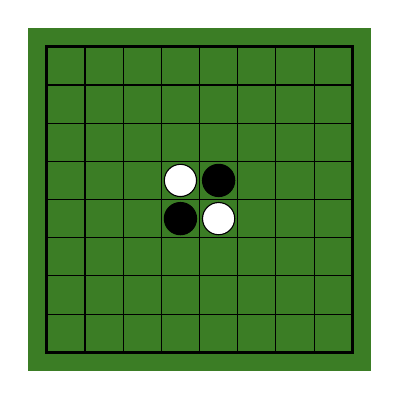
\begin{tikzpicture}[scale=0.485] \tikzstyle{every node}=[font=\small]
			% Draw the background
			\fill[OliveGreen] (-0.5,-0.5) rectangle (8.5,8.5);
			
			% Draw the grid lines
			\draw[step=1cm, black] (0,0) grid (8,8);
			
			% Draw the thick border
			\draw[very thick] (0,0) rectangle (8,8);
			
			% Draw the central black dot
			\filldraw[draw=black,fill=white] (4.5,3.5) circle (12pt);
			\filldraw[draw=black,fill=white] (3.5,4.5) circle (12pt);
			
			
			%\filldraw[Blue] (0,0) circle (6pt);
			\filldraw[black] (3.5,3.5)  circle (12pt);
			\filldraw[black] (4.5,4.5)  circle (12pt);
			
		\end{tikzpicture}
		\caption{Tablero de Othello con su posición inicial.}
		\label{fig:Tab_Othello}
	\end{wrapfigure}
	Si tuviéramos $\Delta_{oth}$, el Othello puede construirse sobre el juego:
	$(N\times N, \{0,1,2\}, A_{ort} \cup A_{diag}, \Delta_{Oth}).$
	Con $|N|=8$, $A_{diag}$ el criterio que toma en cuenta las diagonales $(\pm1,\pm1)$ y $\Delta_{Oth}$ las reglas de cambios en el Othello. De esta manera, la construcción desarrollada sugiere una posible formalización del \textit{Othello} dentro del mismo marco teórico.\hfill\break
	
	\subsection*{Havannah}
	
	\begin{wrapfigure}[13]{r}{0.35\textwidth}
		\centering
		\begin{tikzpicture}[scale=0.485] \tikzstyle{every node}=[font=\small]
			
			% Parámetros del hexágono
			\def\r{0.58}
			
			% Función para dibujar una celda hexagonal
			\foreach \q in {-4,...,4}{
				\pgfmathtruncatemacro{\rmin}{max(-4,-\q-4)}
				\pgfmathtruncatemacro{\rmax}{min(4,-\q+4)}
				\foreach \s in {\rmin,...,\rmax}{
					\pgfmathsetmacro{\x}{0.575*sqrt(3)*(\q+\s/2)}
					\pgfmathsetmacro{\y}{0.575*1.5*\s}
					
					\draw[fill=goban]
					(\x,\y)
					++(30:\r)
					\foreach \a in {90,150,210,270,330}{
						-- ++(\a:\r)
					} -- cycle;
				}
			}
			
			% ------------------------
			% Anillo (azul)
			% ------------------------
			
			\foreach \q/\s in {
				0/1,1/0,1/-1,0/-1,-1/0,-1/1, -1/1
				%				0/2,2/0,2/-2,0/-2,-2/0,-2/2
			}{
				\pgfmathsetmacro{\x}{0.575*sqrt(3)*(\q+\s/2)}
				\pgfmathsetmacro{\y}{0.575*1.5*\s}
				
				\filldraw[fill=Blue]
				(\x,\y)
				++(30:\r)
				\foreach \a in {90,150,210,270,330}
				{ -- ++(\a:\r) } -- cycle;
			}
			
			% ------------------------
			% Puente (rojo)
			% ------------------------
			
			\foreach \q/\s in {
				-4/0, 	-3/0, -3/1,-3/2,-3/3,-4/4
			}{
				\pgfmathsetmacro{\x}{0.575*sqrt(3)*(\q+\s/2)}
				\pgfmathsetmacro{\y}{0.575*1.5*\s}
				
				\filldraw[fill=Red]
				(\x,\y)
				++(30:\r)
				\foreach \a in {90,150,210,270,330}
				{ -- ++(\a:\r) } -- cycle;
			}
			
			% ------------------------
			% Tenedor (verde)
			% ------------------------
			
			\foreach \q/\s in {
				1/-2, 2/-2,3/-2, 3/-2, 
				1/-3, 1/-4,
				3/-1, 4/-2, 3/0, 3/1
			}{
				\pgfmathsetmacro{\x}{0.575*sqrt(3)*(\q+\s/2)}
				\pgfmathsetmacro{\y}{0.575*1.5*\s}
				
				\filldraw[fill=OliveGreen]
				(\x,\y)
				++(30:\r)
				\foreach \a in {90,150,210,270,330}
				{ -- ++(\a:\r) } -- cycle;
			}
		\end{tikzpicture}
		\caption{Las tres estructuras ganadoras en el Havannah: \textcolor{Blue}{anillo}, \textcolor{Red}{puente} y \textcolor{OliveGreen}{tenedor}.}
		\label{fig:havannah}
	\end{wrapfigure}
	Otro ejemplo interesante es el Havannah. A diferencia del Go, este juego se desarrolla sobre un tablero hexagonal y las piedras son adyacentes según la geometría propia de dicho tablero. Nuevamente, basta modificar el criterio de adyacencia. La particularidad del Havannah es que existen tres formas distintas de ganar: construir un \textcolor{Blue}{anillo}, un \textcolor{Red}{puente} o un \textcolor{OliveGreen}{tenedor}, véase Figura~\ref{fig:havannah}.
	
	Nuestra teoría ya contempla el caso del \textcolor{Blue}{anillo}. En efecto, un anillo es simplemente un grupo que encierra una región. Si distinguimos las seis esquinas del tablero como subconjuntos especiales de posiciones, un \textcolor{Red}{puente} puede describirse como un grupo que contiene piedras en al menos dos esquinas distintas. Del mismo modo, si distinguimos los seis bordes del tablero, un \textcolor{OliveGreen}{tenedor} puede describirse como un grupo que contiene piedras en al menos tres bordes distintos.
	
	Si recordamos las propiedades de $|K(i)|$ discutidas en la Parte~\ref{parte1} esto nos basta para poder identificar qué puntos pertenecen a las esquinas o bordes, Sección~\ref{posicion_espacial}. De esta manera, la condición de victoria del Havannah puede expresarse únicamente en términos de grupos, regiones y subconjuntos del tablero. En consecuencia, el juego parece admitir una formalización natural dentro del mismo marco teórico.
	\subsection*{Hex}
	\begin{wrapfigure}[12]{i}{0.47\textwidth}
		\centering
		\begin{tikzpicture}[scale=0.4]
			\def\r{0.55}
			
			%% Borde de colores de cada jugador
			\coordinate (TL) at (4.2,9.7);
			\coordinate (TR)at (16,9.7);
			\coordinate (BL) at (-1.5,-0.35);
			\coordinate (BR) at (10,-0.35);
			\coordinate (C) at (7,5);
			
			\fill[Blue] (TL) -- (C) -- (TR) -- cycle;
			\fill[Blue] (BL) -- (C) -- (BR) -- cycle;
			
			\fill[Red] (TL) -- (C) -- (BL) -- cycle;
			\fill[Red] (TR) -- (C) -- (BR) -- cycle;
			\draw[thick] (TL)--(TR)--(BR)--(BL)--cycle;
			
			
			% Tablero 11x11 tipo Hex
			\foreach \i in {0,...,10}{
				\foreach \j in {0,...,10}{
					
					\pgfmathsetmacro{\x}{0.55*sqrt(3)*(\i+\j/2)}
					\pgfmathsetmacro{\y}{0.55*1.5*\j}
					
					\draw[fill=goban]
					(\x,\y)
					++(30:\r)
					\foreach \a in {90,150,210,270,330}
					{ -- ++(\a:\r)}
					-- cycle;
				}
			}
			
			
			
			\foreach \i/\j in {
				0/5, 1/5, 2/5, 2/6,	3/6,
				4/6, 5/6, 6/6, 6/7, 7/7,
				8/7, 8/8, 9/8, 10/8
			}
			{ 
				\pgfmathsetmacro{\x}{0.55*sqrt(3)*(\i+\j/2)}
				\pgfmathsetmacro{\y}{0.55*1.5*\j}
				\filldraw[fill=Red] (\x,\y) ++(30:\r) \foreach \a in {90,150,210,270,330} { -- ++(\a:\r)} -- cycle; }
		\end{tikzpicture}
		\caption{\textcolor{Red}{Cadena} ganadora que conecta dos bordes opuestos.}
		\label{fig:hex}
	\end{wrapfigure}
	Consideremos ahora el Hex, Figura~\ref{fig:hex}. El tablero es hexagonal, basta adaptar el criterio de adyacencia. A diferencia del Go, en Hex no existen capturas. Para ganar se tiene que construir un camino de una esquina a su opuesta. Basta distinguir los bordes opuestos del tablero como subconjuntos de posiciones, la condición de victoria puede expresarse de manera muy sencilla: un jugador gana si existe un grupo de su color que interseca ambos bordes opuestos de su color. Así, la victoria en Hex se reduce a una propiedad de los grupos.
	
	\subsection*{El juego de Shannon}
	
	El Juego de Shannon constituye un ejemplo particularmente interesante, a diferencia del Go, Hex o Havannah, no se desarrolla sobre un tablero, sino, sobre un grafo finito arbitrario. Los jugadores que son dos, alternan turnos, el jugador Short toma una arista del grafo y la colorea, Cut toma una arista del grafo y la elimina. Short vence si sus aristas elegidas contiene un camino que conecta los vértices distinguidos $A$ y $B$. Cut gana si logra desconectar los vértices $A$ y $B$.
	\begin{figure}[H]
		\centering
		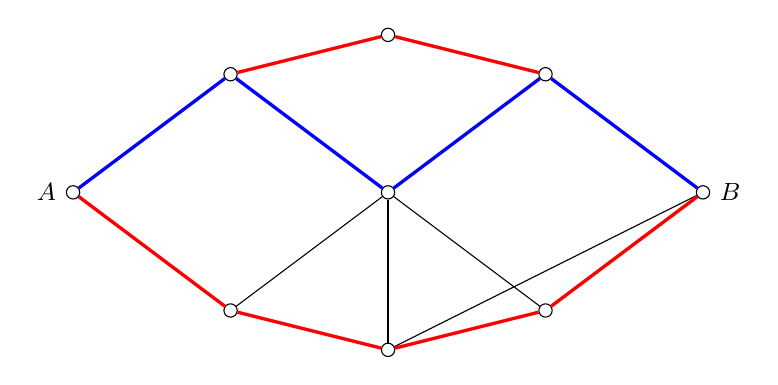
\begin{tikzpicture}[
			scale=1,
			vertex/.style={circle,draw,fill=white,inner sep=1.7pt}
			]
			
			% Vértices
			\node[vertex,label=left:$A$] (A) at (0,0) {};
			\node[vertex] (v1) at (2,1.5) {};
			\node[vertex] (v2) at (2,-1.5) {};
			\node[vertex] (v3) at (4,2) {};
			\node[vertex] (v4) at (4,0) {};
			\node[vertex] (v5) at (4,-2) {};
			\node[vertex] (v6) at (6,1.5) {};
			\node[vertex] (v7) at (6,-1.5) {};
			\node[vertex,label=right:$B$] (B) at (8,0) {};
			% Aristas libres (negras)
			\draw (v2)--(v4);
			\draw (v4)--(v5);
			\draw (v4)--(v7);
			\draw (v5)--(B);
			\draw (v3)--(v6);
			% Aristas de Short (azules)
			\draw[very thick,Blue] (A)--(v1);
			\draw[very thick,Blue] (v1)--(v4);
			\draw[very thick,Blue] (v4)--(v6);
			\draw[very thick,Blue] (v6)--(B);
			
			% Aristas de Cut (rojas)
			\draw[very thick,Red] (A)--(v2);
			\draw[very thick,Red] (v2)--(v5);
			\draw[very thick,Red] (v5)--(v7);
			\draw[very thick,Red] (v7)--(B);
			
			\draw[very thick,Red] (v1)--(v3);
			\draw[very thick,Red] (v6)--(v3);
			
			
			
		\end{tikzpicture}
		\caption{Las aristas azules pertenecen a Short, las rojas a Cut y las negras permanecen libres. El conjunto de aristas azules determina un camino entre los vértices distinguidos $A$ y $B$, por lo que Short gana.}
	\end{figure}
	
	Sea $G=(V,E)$ un grafo finito y sean $A,B\in V$ dos vértices distinguidos. Consideraremos cada arista del grafo como una posición jugable. En consecuencia, el conjunto de posiciones vendrá dado por $T=E$. Los estados posibles de una posición serán $E_s=\{0,1,2\}$,	donde $0$ representa una arista libre, $1$ una arista controlada por Short y $2$ una arista controlada por Cut.
	
	Definimos una relación de adyacencia $T_s$ sobre $T$, dos posiciones $e_1,e_2\in T$ son adyacentes cuando las aristas correspondientes comparten un vértice, es decir,
	$$	e_1\sim e_2	\iff e_1\cap e_2\neq\varnothing.$$
	Con esta definición, los grupos introducidos anteriormente coinciden con componentes conexas de aristas de un mismo color. Denotamos la dinámica del juego por $\Delta_s$, cualquier Juego de Shannon asociado al grafo $G$ puede representarse mediante la estructura:
	$$(T,E_s,T_s,\Delta_s).$$
	Este ejemplo resulta especialmente revelador, pues muestra que la estructura desarrollada no depende de nociones geométricas como regiones o territorios. Aun tratándose de un juego definido sobre un grafo arbitrario, las nociones de posición, estado, adyacencia y grupo siguen siendo suficientes para describir completamente su dinámica. Parece ser que la teoría desarrollada no describe únicamente al Go, sino a una familia más amplia de juegos, los \emph{Juegos de Rodear} $(\mathsf{JR})$.\footnote{Este nombre no es correcto pero, es el que surgió durante el desarrollo. Se adopta aquí por conveniencia y no pretende identificar una matemática establecida. La determinación de una denominación adecuada requeriría un estudio más amplio.}
	%	por lo tanto, $Othello \in \textsf{JR}$.
	%	\begin{figure}[H]
		%		\centering
		%		\begin{tikzpicture}[
			%			node distance=2.5cm and 3cm,
			%			game/.style={circle, draw=black, thick, fill=white, minimum size=1.2cm, font=\large},
			%			cat/.style={circle, fill=gray!20, draw=black, very thick, minimum size=1.5cm, font=\large\bfseries},
			%			morphism/.style={->, thick},
			%			label/.style={font=\footnotesize, align=center}
			%			]
			%			
			%			% Nodo Principal (La Categoría)
			%			\node[cat] (C) {\textsf{JR}};
			%			
			%			% Nivel 1: Juegos Base
			%			\node[game, below left=2cm and 2cm of C] (J1) {$J_1$};
			%			\node[game, below right=2cm and 2cm of C] (J2) {$J_2$};
			%			
			%			% Flechas de pertenencia/inclusión a la categoría (Opcional, punteadas)
			%			\draw[->, dashed, gray, thick] (C) -- node[above left, font=\scriptsize, text=gray] {obj} (J1);
			%			\draw[->, dashed, gray, thick] (C) -- node[above right, font=\scriptsize, text=gray] {obj} (J2);
			%			
			%			% Morfismos entre J1 y J2 (Cambio de Reglas - Delta)
			%			\draw[<->, Blue, thick] (J1) to[bend left=15] node[above, label, text=Blue] {Cambia $\Delta$\\$f: \Delta_1 \to \Delta_2$} (J2);
			%			
			%			% Ramificaciones desde J1 (Derivaciones)
			%			\node[game, draw=Red, text=Red, below left=2.5cm and 1cm of J1] (J1A) {$J'_1$};
			%			\node[game, draw=OliveGreen!50!black, text=OliveGreen!50!black, below right=2.5cm and 1cm of J1] (J1GE) {$J''_1$};
			%			
			%			% Morfismos desde J1
			%			\draw[morphism, Red] (J1) -- node[above left, label, text=Red] {Cambia $A$\\$A_1 \to A_2$} (J1A);
			%			\draw[morphism, OliveGreen!50!black] (J1) -- node[above right, label, text=OliveGreen!50!black] {Cambia $G,E$\\$(G_1,E_1) \to (G_2,E_2)$} (J1GE);
			%			
			%			% Ramificaciones desde J2 (Derivaciones)
			%			\node[game, draw=Red, text=Red, below left=2.5cm and 1cm of J2] (J2A) {$J'_2$};
			%			\node[game, draw=OliveGreen!50!black, text=OliveGreen!50!black, below right=2.5cm and 1cm of J2] (J2GE) {$J''_2$};
			%			
			%			% Morfismos desde J2
			%			\draw[morphism, Red] (J2) -- node[above left, label, text=Red] {} (J2A);
			%			\draw[morphism, OliveGreen!50!black] (J2) -- node[above right, label, text=OliveGreen!50!black] {} (J2GE);
			%			
			%		\end{tikzpicture}
		%		\caption{Estructura de la categoría $\textsf{JR}$. El nodo raíz representa la categoría que contiene a los juegos como objetos. Entre $J_1$ y $J_2$ existe un morfismo que altera sus reglas de captura ($\Delta$). De estos juegos se derivan otros mediante morfismos que alteran sus relaciones ($A$) produciendo $J'$, o bien su espacio y jugadores ($G, E$) produciendo $J''$.}
		%		\label{fig:esquema_arbol}
		%	\end{figure}
	\newpage
	%\section*{Glosario (Parte III)}
	%\begin{center}
	%	\begin{tabular}{p{2cm} p{4.7cm} p{2cm} p{4.7cm}}
		%		\toprule
		%		\textbf{Símbolo} & \textbf{Significado} & \textbf{Símbolo} & \textbf{Significado} \\
		%		\midrule
		%		$A(x,y,z)_\beta$ & Adyacencias del exterior 3D & $\tilde{A}(x,y,z)_\theta$ & Promedio de adyacencias del exterior 3D \\
		%		$A(x,y)_\tau$ & Adyacencias del tablero toroidal 2D & $\tau$ & Transformación toroidal (unión de bordes opuestos) \\
		%		$\partial G$ & Frontera del tablero (puntos en bordes) & $\varphi$ & Inmersión en una dimensión extra ($g\mapsto(g,1)$) \\
		%		$\Xi$ & Expansión con un conjunto $M$ ($g\mapsto(g,m)$) & $\iota$ & Inclusión de un nuevo jugador ($E\mapsto E\cup\{y\}$) \\
		%		$U$ & Proyección & & \\
		%		\bottomrule
		%	\end{tabular}
	%\end{center}